\documentclass[conference]{IEEEtran}
\IEEEoverridecommandlockouts
% The preceding line is only needed to identify funding in the first footnote. If that is unneeded, please comment it out.
% Template version as of 6/27/2024

\usepackage{cite}
\usepackage{amsmath,amssymb,amsfonts}
\usepackage{url}
\usepackage{algorithmic}
\usepackage{graphicx}
\usepackage{textcomp}
\usepackage{xcolor}
\usepackage{float}
\def\BibTeX{{\rm B\kern-.05em{\sc i\kern-.025em b}\kern-.08em
T\kern-.1667em\lower.7ex\hbox{E}\kern-.125emX}}

\begin{document}

\title{Inferno Tactics\\
% {\footnotesize \textsuperscript{*}Note: Sub-titles are not captured for [https://ieeexplore.ieee.org](https://ieeexplore.ieee.org) and
% should not be used}
}

\author{\IEEEauthorblockN{1\textsuperscript{st} Shaurya Mathur}
\IEEEauthorblockA{\textit{Dept. of Computer Science \& Engineering} \\
\textit{University at Buffalo}\\
Buffalo, USA \\
smathur4@buffalo.edu}
\and
\IEEEauthorblockN{2\textsuperscript{nd} Shreyas Bellary Manjunath}
\IEEEauthorblockA{\textit{Dept. of Computer Science \& Engineering} \\
\textit{University at Buffalo}\\
Buffalo, USA \\
sbellary@buffalo.edu}
}

\maketitle

\begin{abstract}
Inferno Tactics presents a novel integrated approach to wildfire management that combines Deep Learning (DL) prediction capabilities with Reinforcement Learning (RL) mitigation strategies. Our system employs a two-phase architecture: first, a deep learning model analyzes historical wildfire patterns and Earth Engine satellite imagery to forecast potential ignition events with precise geographic and temporal specifications. Building upon these predictions, our custom-built 3D simulation environment reconstructs terrain and vegetation conditions from actual geodata, enabling realistic wildfire spread modeling. Within this environment, we've developed and trained a helitack agent using Proximal Policy Optimization (PPO) that demonstrates effective firefighting capabilities through strategic water deployment. The agent successfully learns to prioritize active fire fronts, establish firebreaks in high-risk zones, and efficiently allocate limited resources. Our web application provides an intuitive interface for emergency personnel to input coordinates and receive not only wildfire predictions but also visualized mitigation simulations with actionable strategies.
While still under active development, preliminary results suggest that the RL-enhanced validation significantly improves the system's ability to filter out false positives and deliver timely alerts for disaster management.
\end{abstract}

\begin{IEEEkeywords}
wildfire, gym, deep learning, reinforcement learning
\end{IEEEkeywords}

\section{Introduction}

Wildfires are increasingly becoming a global threat, with rising temperatures and shifting climate patterns contributing to their frequency and intensity. These fires not only devastate ecosystems but also endanger human lives and infrastructure. Traditional methods of wildfire detection and response often rely on environmental monitoring and sensor-based data; however, these approaches are largely reactive and struggle to provide timely and strategic interventions over vast, unmonitored regions.

\noindent
\textit{Inferno Tactics} explores a novel approach that integrates Deep Learning (DL) with Reinforcement Learning (RL) to both predict and plan for wildfire events. The DL component analyzes satellite imagery and historical wildfire data to forecast the time and location of potential wildfire outbreaks. In parallel, the RL component simulates a dynamic environment where wildfires may occur, allowing an intelligent agent to learn optimal mitigation strategies through trial-and-error interactions. These strategies can involve decisions such as resource deployment, early evacuation planning, or the prioritization of firebreak construction.

\noindent
By modeling wildfire scenarios as a Markov Decision Process (MDP), the RL agent learns to make sequential decisions that aim to minimize long-term damage. This dual-system framework—combining predictive modeling with adaptive planning—seeks to enable a more proactive and automated wildfire management system.

\noindent
This report presents the implementation and results of the project, including detailed descriptions of the geospatial data acquisition pipeline, simulation environment, and reinforcement learning training framework. We demonstrate the feasibility of combining DL and RL for improving wildfire prediction, verification, and strategic response planning.

\section{Background and Motivation}

\subsection{Wildfires and the Need for Intelligent Response}
Wildfires are becoming increasingly destructive due to climate change, land-use patterns, and prolonged dry seasons. Traditional wildfire response mechanisms, while valuable, often rely on reactive strategies that lack foresight and scalability. In the face of rapidly spreading fires, there's a growing need for proactive and intelligent systems that not only predict the likelihood of wildfires but also simulate and learn effective mitigation responses in real-time.

\subsection{Simulating Wildfire Behavior with Real-World Data}
To study wildfire dynamics in a realistic setting, we have developed an interactive simulation environment using \texttt{React.js} and \texttt{three.js}. This simulation serves as a visual and behavioral model of wildfire propagation, incorporating real-world geographic data to enhance its accuracy.

\noindent
Specifically, we use Google Earth Engine APIs to fetch terrain elevation and land cover data, which are then integrated into the simulation. These attributes—along with wind speed and direction—play a crucial role in shaping how fire spreads. By grounding the simulation in actual Earth data, we aim to mimic plausible wildfire scenarios that are both visually intuitive and spatially accurate.

\subsection{Modeling Firefighting Agents via Reinforcement Learning}
At the core of our project is a Reinforcement Learning (RL) agent designed to develop and optimize wildfire mitigation strategies. We connect our React-based frontend to a custom Python-based \texttt{Gym} environment via WebSockets, enabling real-time interaction between the simulation and the RL backend.

\noindent
The initial agent we have developed simulates a \textit{helitack} unit—a helicopter-based firefighting strategy. As part of our future work, we plan to implement additional agent types such as ground crews, fire trucks, and fixed-wing aircraft to create a more comprehensive firefighting simulation. Using the \texttt{Stable Baselines3} library, we train the helitack agent to explore and learn optimal policies to suppress fires efficiently across different terrain and wind conditions. The agent's goal is to minimize the spread and damage caused by the fire over time, adapting its actions based on changing environmental dynamics.

\subsection{Motivation for Hierarchical Multi-Agent Planning}
While the helitack strategy is effective in certain scenarios, real-world wildfire mitigation often involves a combination of approaches, including fire trucks, aerial water drops, and firebreak construction. To simulate such complexity, we plan to extend our system using \textit{Hierarchical Reinforcement Learning (HRL)}.

\noindent
In this framework, high-level policies will determine which mitigation strategy (e.g., helitack, fire truck dispatch) to deploy, while lower-level agents execute specialized tasks based on the chosen strategy. This modular architecture enables coordinated planning, resource allocation, and scalable learning across different fire response techniques.

\noindent
Our motivation stems from building a generalized, adaptable simulation tool that can train agents capable of multi-modal disaster response. By modeling realistic wildfire environments and training agents through trial-and-error, we aim to develop an intelligent system that can assist human decision-makers in planning efficient, timely, and context-aware fire mitigation strategies.

\section{Geodata Extraction and Processing}

A critical component of our system is the ability to model realistic wildfire scenarios using actual geographical data. To achieve this, we developed a comprehensive geodata extraction pipeline that sources, processes, and transforms Earth observation data into simulation-ready assets.

\subsection{Google Earth Engine Integration}
We implemented a Python module that interfaces with the Google Earth Engine API to extract two primary types of data:

\begin{itemize}
    \item \textbf{Elevation Data:} Digital Elevation Models (DEMs) from the Shuttle Radar Topography Mission (SRTM) dataset, providing terrain height information at 30-meter resolution globally.
    \item \textbf{Land Cover Data:} MODIS land cover dataset, which classifies land into distinct categories including forests, grasslands, urban areas, and water bodies.
\end{itemize}

\noindent
The extraction process begins with a set of predicted wildfire ignition coordinates (latitude and longitude) obtained from our deep learning prediction module. These coordinates serve as the center point for a regional extraction, typically covering a 10km × 10km area.

\subsection{Data Processing Pipeline}
Our geodata processing workflow consists of several stages:

\begin{enumerate}
    \item \textbf{API Request and Authentication:} Secure authentication with Earth Engine servers and formulation of data retrieval requests based on geographical bounds.
    \item \textbf{Resolution Harmonization:} Resampling of disparate data sources to ensure consistent spatial resolution across datasets.
    \item \textbf{GeoTIFF Generation:} Export of processed data as GeoTIFF files, preserving both the raw data values and geospatial metadata.
    \item \textbf{Heightmap Conversion:} Transformation of elevation GeoTIFFs into grayscale heightmap PNG images, where pixel intensity corresponds to elevation.
    \item \textbf{Land Cover Reclassification:} Mapping of MODIS land cover classes to simulation-relevant fire behavior parameters (e.g., fuel load, ignition probability).
\end{enumerate}

\begin{figure}[h!]
\centering
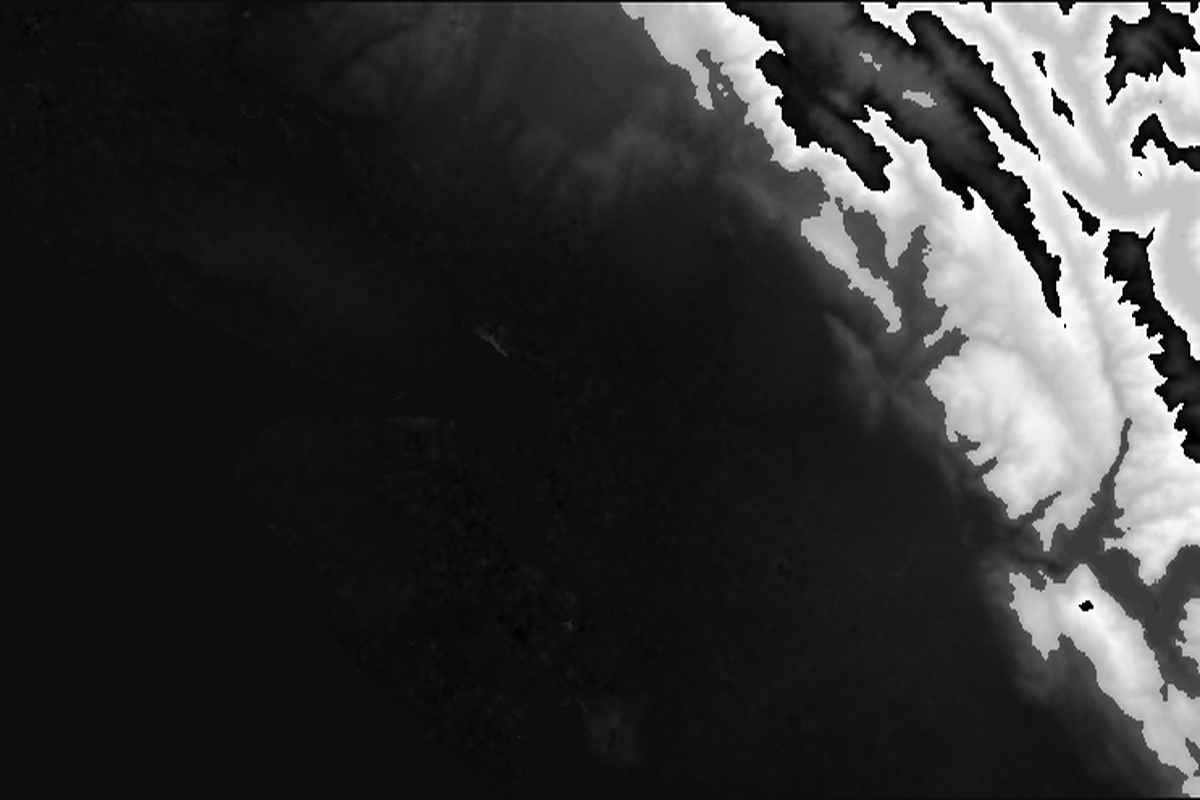
\includegraphics[width=0.5\textwidth]{heightmap.png}
\caption{Heightmap generated from SRTM elevation data, with pixel intensity representing terrain elevation.}
\end{figure}

\subsection{Simulation Environment}
The processed geodata serves as the foundational layer for our simulation environment:

\begin{itemize}
    \item Heightmaps are used by Three.js to generate 3D terrain meshes with accurate elevation profiles.
    \item Land cover rasters inform the simulation's fuel model parameters, affecting fire intensity and spread rates.
    \item Additional derived layers (e.g., slope, aspect) are calculated to enhance fire behavior modeling.
\end{itemize}

\noindent
Our current implementation uses a grid size of 1200×800 cells, representing a physical area of 120,000×80,000 meters with a maximum elevation of 10,000 meters. For computational efficiency during development and testing, we also maintain a lower-resolution option with a grid width of 240 cells. By automating this entire pipeline, our system can quickly generate simulation environments for any wildfire-prone region globally, enabling both targeted training scenarios and rapid response simulations for newly predicted wildfire events.

\section{Simulation Environment Development}

\subsection{Three-Dimensional Visualization Framework}
To provide an intuitive and realistic representation of wildfire dynamics, we developed a browser-based simulation environment using \texttt{React.js} for the application framework and \texttt{Three.js} for 3D graphics rendering. This environment serves dual purposes: (1) providing human operators with a visual interface to understand wildfire behavior and intervention effects, and (2) generating visual and numerical data to train reinforcement learning agents.

\begin{figure}[h!]
\centering
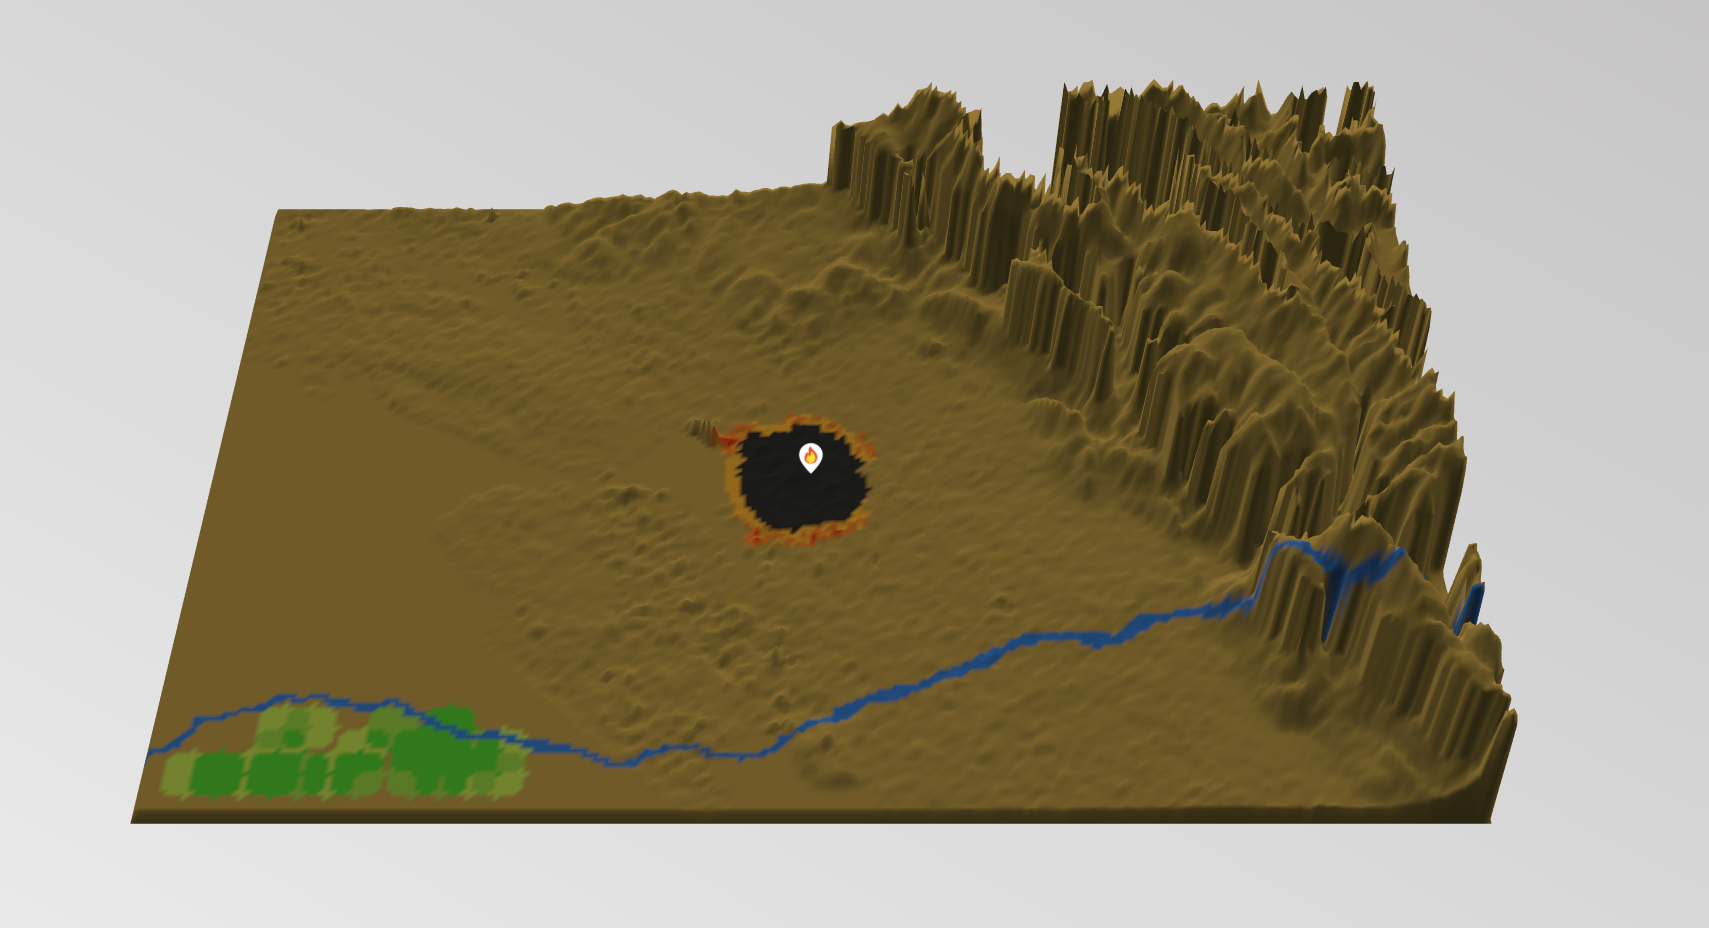
\includegraphics[width=0.5\textwidth]{sim.png}
\caption{Interactive 3D wildfire simulation environment developed in Three.js.}
\end{figure}

\noindent
The visualization framework includes several key components:

\begin{itemize}
    \item \textbf{Terrain Renderer:} Converts heightmap data into a detailed 3D mesh with accurate elevation profiles. The renderer applies texture mapping based on land cover classification to visually differentiate between forests, grasslands, urban areas, and other terrain types.
    
    \item \textbf{Fire Propagation Visualizer:} Implements a particle system and custom shaders to represent active fire fronts, burn intensity, and smoke dispersion. The visual intensity of fire correlates with the underlying fire behavior model's calculated heat release rate.
    
    \item \textbf{Agent Visualization:} Renders firefighting units (e.g., helicopters, ground crews) as interactive 3D models that respond to agent decisions in real-time. Movement paths and action effects (e.g., water drops) are visualized to provide interpretability of agent behavior.
\end{itemize}

\subsection{Fire Behavior Modeling}
At the core of our simulation is a cellular automaton-based fire spread model that calculates fire propagation based on physical and environmental factors:

\begin{itemize}
    \item \textbf{Ignition Time Calculation:} Our model computes the ignition probability and timing for each cell using a comprehensive algorithm that integrates multiple environmental variables:
    \begin{itemize}
        \item Cell moisture content derived from recent precipitation data
        \item Vegetation type and density from MODIS land cover classification
        \item Terrain elevation and slope gradients affecting fuel preheating
        \item Wind speed and direction influencing heat transfer between cells
        \item Ambient temperature and relative humidity affecting fuel dryness
    \end{itemize}
    
    \item \textbf{Fire Intensity Dynamics:} Each cell's burning intensity is calculated on a continuous scale rather than binary states, allowing for more nuanced fire behavior:
    \begin{itemize}
        \item Low, medium, and high intensity states determined by fuel load and environmental conditions
        \item Variable heat release rates affecting neighboring cell ignition probabilities
        \item Intensity-dependent flame height calculations impacting long-distance ember transport
        \item Diurnal temperature variations affecting intensity fluctuations throughout simulated time
    \end{itemize}
    
    \item \textbf{Fuel Consumption Model:} Each cell maintains a dynamically updated fuel state that evolves as the fire progresses:
    \begin{itemize}
        \item Differentiated consumption rates based on fuel type (grass burns faster than forest)
        \item Moisture-dependent burn efficiency affecting heat output and duration
        \item Residual heat calculations that maintain cell temperature after active burning ceases
        \item Fuel depletion thresholds that trigger state transitions from burning to burnt
    \end{itemize}
    
    \item \textbf{Strategic Fire Suppression:} Our current implementation focuses exclusively on helitack operations:
    \begin{itemize}
        \item Water drops create cooling zones with radius proportional to drop intensity
        \item Suppression effectiveness varies based on fire intensity and fuel characteristics
        \item Strategic placement is critical with limited water resources and refill requirements
        \item Our RL agent learns to prioritize containment lines and high-risk spread vectors rather than targeting the most intense portions of the fire
    \end{itemize}
\end{itemize}

\section{Reinforcement Learning Training Framework}

\subsection{Custom OpenAI Gym Environment Implementation}

We developed a custom OpenAI Gym environment that formalizes the wildfire mitigation task as a reinforcement learning problem. This environment implements the standard Gymnasium interface while incorporating the complex dynamics of our wildfire simulation through a WebSocket connection to our React-based frontend:

\begin{itemize}
    \item \textbf{Observation Space:} The agent receives multi-dimensional observations structured as a dictionary:
    \begin{itemize}
        \item \textit{helicopter\_coord}: Box space containing the agent's x,y position (range 0-239, 0-159)
        \item \textit{cells}: A 4-channel grid (160×240) representing stacked frames of the environment state, where each cell's value encodes both fire state (unburnt, burning, burnt) and intensity level (low, medium, high)
        \item \textit{on\_fire}: Binary indicator of whether any cell in the environment is currently burning
    \end{itemize}
    
    \item \textbf{Action Space:} The helitack agent can perform five discrete actions:
    \begin{itemize}
        \item Move in four cardinal directions at a fixed speed (HELICOPTER\_SPEED=3)
        \item Perform a water drop operation at the current location
    \end{itemize}
    
    \item \textbf{Reward Function:} Our reward mechanism incorporates multiple components to guide the agent toward effective firefighting strategies:
    \begin{itemize}
        \item +10 reward for each cell directly extinguished by helitack action
        \item -5 penalty for each newly burnt cell (discouraging fire spread)
        \item -0.1 penalty per burning cell (proportional to current fire size)
        \item -0.1 time penalty to encourage efficient action
        \item Proximity rewards based on distance to nearest fire (2 × e\textsuperscript{-distance/20})
        \item Intensity-based bonuses for targeting high-intensity fires (up to 3× multiplier)
        \item Strategic firebreak rewards for preventive water drops near burning areas
        \item Penalties for wasteful drops on already burnt (-5) or far-from-fire unburnt areas (-10)
    \end{itemize}

    
    \item \textbf{Frame Stacking:} To enable the agent to perceive fire dynamics and spread patterns:
    \begin{itemize}
        \item Environment maintains a history of 4 consecutive frames
        \item New observations replace the oldest frame using an efficient rolling algorithm
        \item This temporal context allows the agent to infer fire movement direction and speed
    \end{itemize}
    
    \item \textbf{Episode Termination:} Episodes conclude when either:
    \begin{itemize}
        \item Fire is completely extinguished (cellsBurning = 0)
        \item Maximum time steps are reached (MAX\_TIMESTEPS = 2000)
    \end{itemize}
\end{itemize}


\subsection{Client-Server Architecture via WebSockets}

To enable real-time communication between the Three.js visualization frontend and the Python-based RL backend, we implemented a bidirectional WebSocket communication layer:

\begin{itemize}
    \item \textbf{Server Component:} A Python server using the \texttt{websockets} library acts as the bridge between the Gym environment and the visualization client. The server:
    \begin{itemize}
        \item Broadcasts environment state updates to connected clients
        \item Receives user interactions or agent actions from clients
        \item Synchronizes simulation time steps across components
        \item Manages training session state and persistence
    \end{itemize}
    
    \item \textbf{Client Component:} The React application integrates WebSocket client functionality to:
    \begin{itemize}
        \item Render received environment states in the 3D visualization
        \item Transmit user commands or agent decisions to the server
        \item Display real-time training metrics and agent performance statistics
        \item Support observer mode during automated training runs
    \end{itemize}
    
    \item \textbf{Protocol Design:} We defined a structured JSON-based message protocol that:
    \begin{itemize}
        \item Minimizes bandwidth requirements through efficient encoding
        \item Supports partial updates to reduce latency
        \item Includes sequence numbering for reliable ordered delivery
        \item Accommodates both synchronous and asynchronous interaction modes
    \end{itemize}
\end{itemize}

\begin{figure}[h!]
\centering
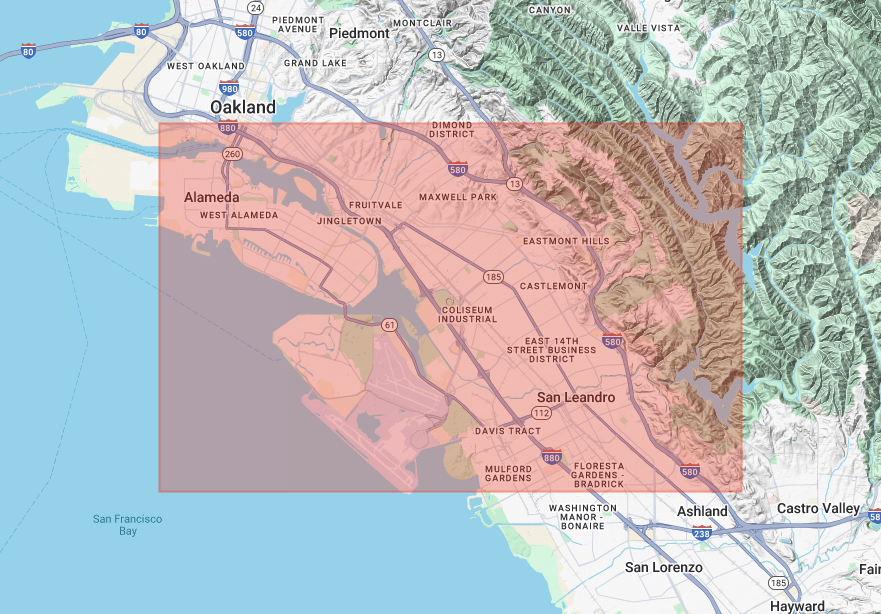
\includegraphics[width=0.5\textwidth]{terrain.png}
\caption{Terrain visualization in the simulation environment, showing elevation and land cover types.}
\end{figure}

\subsection{Neural Architecture for Fire Environment Feature Extraction}

A critical component of our reinforcement learning framework is the custom feature extraction architecture designed specifically for wildfire environments. The spatial complexity and dynamic temporal patterns of fire spread necessitate a specialized neural network that can effectively process multi-scale patterns and temporal sequences. To address this challenge, we developed a multi-faceted feature extraction pipeline:

\subsubsection{Multi-Scale Convolutional Analysis}
Our feature extractor employs a parallel multi-scale CNN approach to simultaneously capture fire dynamics at different spatial resolutions:

\begin{itemize}
    \item \textbf{Small Receptive Field Network:} Processes local fire details with 3×3 kernels, capturing fine-grained burning patterns and precise boundaries between fire states.
    
    \item \textbf{Medium Receptive Field Network:} Identifies fire clusters and potential spread pathways using 5×5 kernels, enabling the agent to recognize emerging fire fronts and strategic intervention points.
    
    \item \textbf{Large Receptive Field Network:} Provides global context with 11×11 and 7×7 kernels, allowing the agent to understand overall fire distribution and macro-level patterns across the terrain.
\end{itemize}

This multi-resolution approach ensures that the agent simultaneously perceives both localized details (which cell is burning at what intensity) and global patterns (overall fire shape and spread direction), mirroring how human firefighters assess wildfire scenarios across different scales.

\subsubsection{Spatial Attention Mechanism}
To focus computational resources on the most relevant regions of the environment, we implemented a spatial attention mechanism that enhances important features:

\begin{itemize}
    \item The attention module generates a pixel-wise weighting map that emphasizes critical areas such as active fire fronts and potential spread vectors.
    
    \item A residual connection (attended features + original features) ensures that no information is lost during the attention process while still highlighting priority regions.
    
    \item This mechanism enables the agent to prioritize actions in high-risk areas without completely ignoring secondary concerns, much like how human firefighters must allocate limited resources to the most critical fire zones.
\end{itemize}

\subsubsection{Temporal Understanding via LSTM}
Fire behavior is inherently temporal, with spread patterns evolving over time based on terrain, wind, and intervention effects. To capture these dynamics:

\begin{itemize}
    \item We incorporate a two-layer LSTM network with 256 hidden units that processes the sequence of observations, enabling the agent to recognize temporal patterns in fire spread.
    
    \item The LSTM maintains internal state between time steps, allowing the agent to develop an understanding of fire momentum, spread rates, and the effectiveness of previous interventions.
    
    \item This recurrent architecture helps the agent anticipate future fire movement rather than simply reacting to the current state, enabling more strategic planning and proactive firefighting.
\end{itemize}

\subsubsection{Coordinate and Fire State Integration}
To complete the agent's situational awareness, we process additional contextual information:

\begin{itemize}
    \item The helicopter's absolute and relative position (distance from center) is encoded through a specialized coordinate network, helping the agent develop an understanding of spatial relationships and egocentric navigation.
    
    \item A binary fire status flag is processed to provide immediate feedback on whether any cells are currently burning, serving as a high-level indicator of mission status.
    
    \item These features are concatenated with the CNN and LSTM outputs to create a comprehensive representation of the environment state.
\end{itemize}

\subsubsection{Integration with PPO Algorithm}
The feature extractor is integrated into our PPO implementation through a custom policy class that connects the extractor to the actor and critic networks:

\begin{itemize}
    \item The actor network maps the extracted features to a probability distribution over the five possible actions (four movement directions and water drop).
    
    \item The critic network estimates the value function from the same features, enabling effective advantage estimation for policy updates.
    
    \item During training, the entire architecture—including the feature extractor—is optimized end-to-end, allowing the perception components to adapt specifically to the wildfire suppression task.
\end{itemize}

\begin{figure}[H]
    \centering
    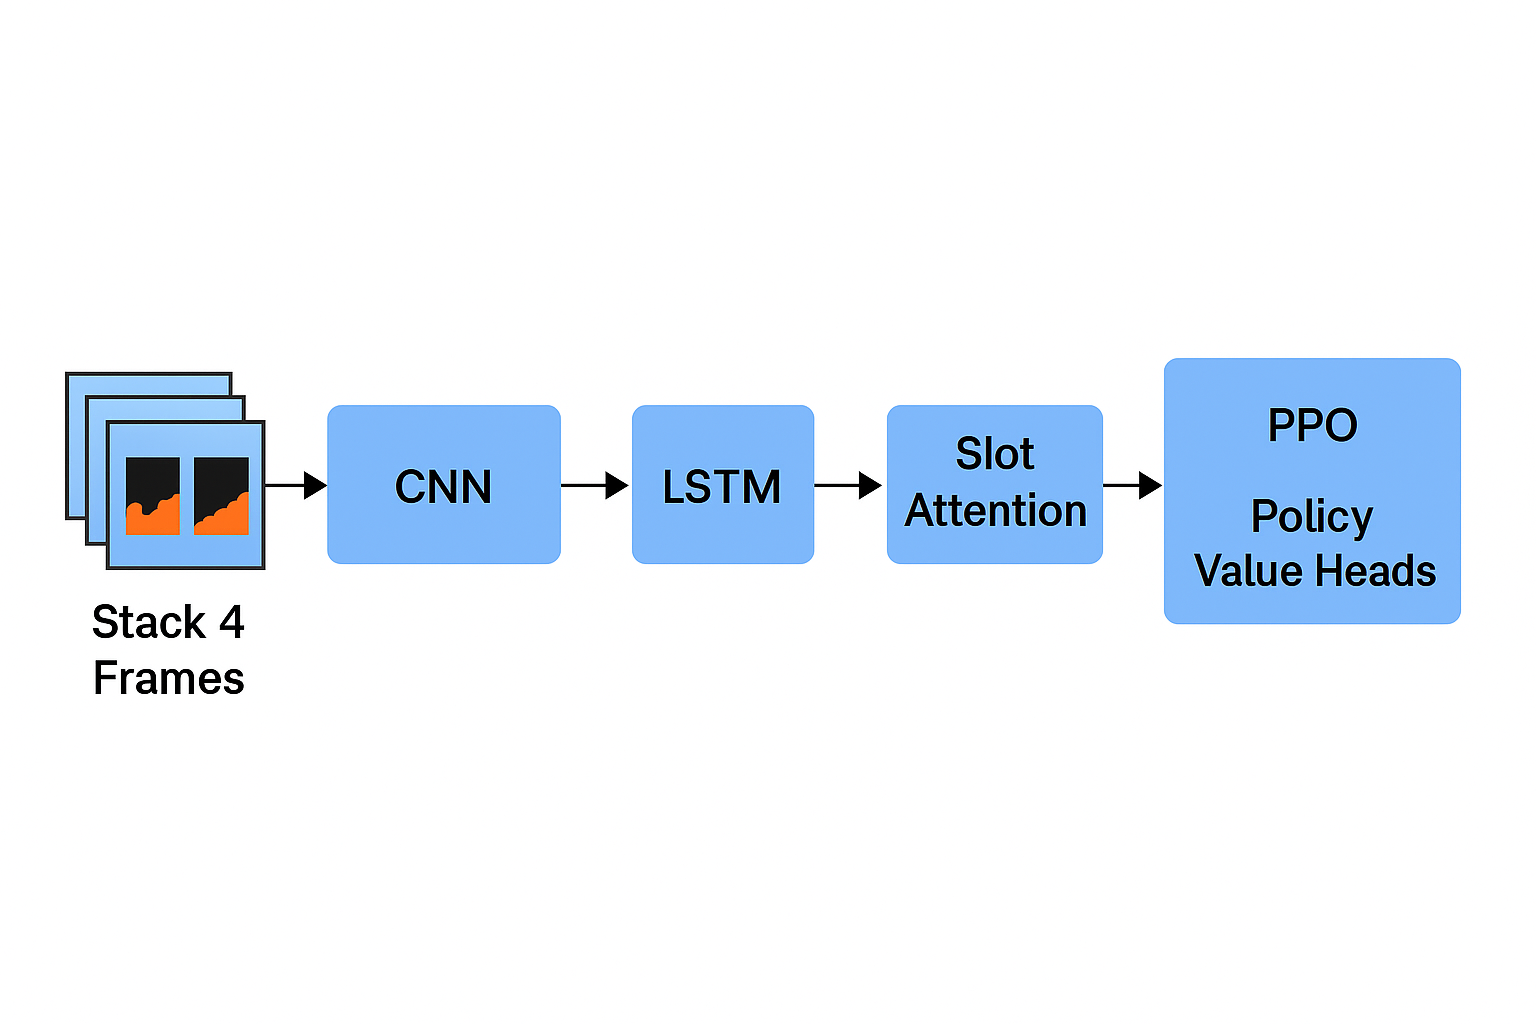
\includegraphics[width=0.5\textwidth]{feat_extr.png}
    \caption{Architecture of our FireEnvLSTMCNN feature extractor with multi-scale convolutional pathways, spatial attention, and LSTM temporal processing.}
    \end{figure}

\subsection{Containerized Training Infrastructure}

To ensure reproducibility and scalability of our training process, we implemented a Docker-based training infrastructure:

\begin{itemize}
    \item \textbf{Containerization:} The entire training stack is encapsulated in Docker containers, including:
    \begin{itemize}
        \item Python environment with RL libraries and dependencies
        \item WebSocket server for communication
        \item React client for visualization (headless mode for training)
        \item Data processing utilities for geodata preparation
    \end{itemize}
    
    \item \textbf{Training Orchestration:} We use Docker Compose to coordinate multiple container instances for:
    \begin{itemize}
        \item Parallel training of multiple agent variants
        \item Hyperparameter optimization runs
        \item Distributed evaluation across different wildfire scenarios
        \item Performance benchmarking and ablation studies
    \end{itemize}
    
    \item \textbf{Resource Management:} The containerized approach enables efficient allocation of computational resources:
    \begin{itemize}
        \item GPU acceleration for neural network training
        \item CPU optimization for simulation physics
        \item Memory management for handling multiple concurrent environments
        \item Easy deployment across different computing platforms
    \end{itemize}
\end{itemize}

\subsection{Reinforcement Learning Algorithm Implementation}

We implemented and evaluated several reinforcement learning algorithms, ultimately selecting Proximal Policy Optimization (PPO) from the Stable Baselines3 library as our primary approach:

\begin{itemize}
    \item \textbf{Policy Network Architecture:} Our implementation uses:
    \begin{itemize}
        \item Convolutional layers to process spatial observation data
        \item Attention mechanisms to focus on critical regions (e.g., active fire fronts)
        \item Recurrent components (LSTM) to model temporal dependencies in fire behavior
        \item Separate value and policy heads for stable learning
    \end{itemize}
    
    \item \textbf{Training Curriculum:} To facilitate efficient learning in this complex domain, we developed a progressive curriculum:
    \begin{itemize}
        \item Initial training on simplified scenarios with single ignition points
        \item Gradual introduction of variable wind conditions
        \item Progression to complex terrain with diverse land cover
        \item Final training on realistic multi-ignition scenarios
    \end{itemize}
    
    \item \textbf{Hyperparameter Optimization:} Key parameters were tuned using grid search and Bayesian optimization:
    \begin{itemize}
        \item Learning rate schedules optimized for stability
        \item PPO clip range tuned to prevent policy collapse
        \item Entropy coefficient adjusted to balance exploration and exploitation
        \item Discount factor (gamma) set to account for delayed effects of firefighting actions
    \end{itemize}
\end{itemize}

\noindent
This comprehensive training framework enables our helitack agent to learn effective wildfire mitigation strategies that adapt to the complex and dynamic nature of fire behavior across diverse geographical and environmental contexts. In future iterations, we plan to extend this framework to support multiple agent types that can operate collaboratively.

\section{Interactive Web Application}

To make our wildfire prediction and mitigation system accessible to a wider audience, we have developed a user-friendly web application that facilitates interaction with our trained models. This interface serves as a bridge between the technical complexity of the AI models and the practical needs of emergency management personnel.

\subsection{User Interface and Workflow}
The web application provides an intuitive interface where users can:

\begin{figure}[H]
    \centering
    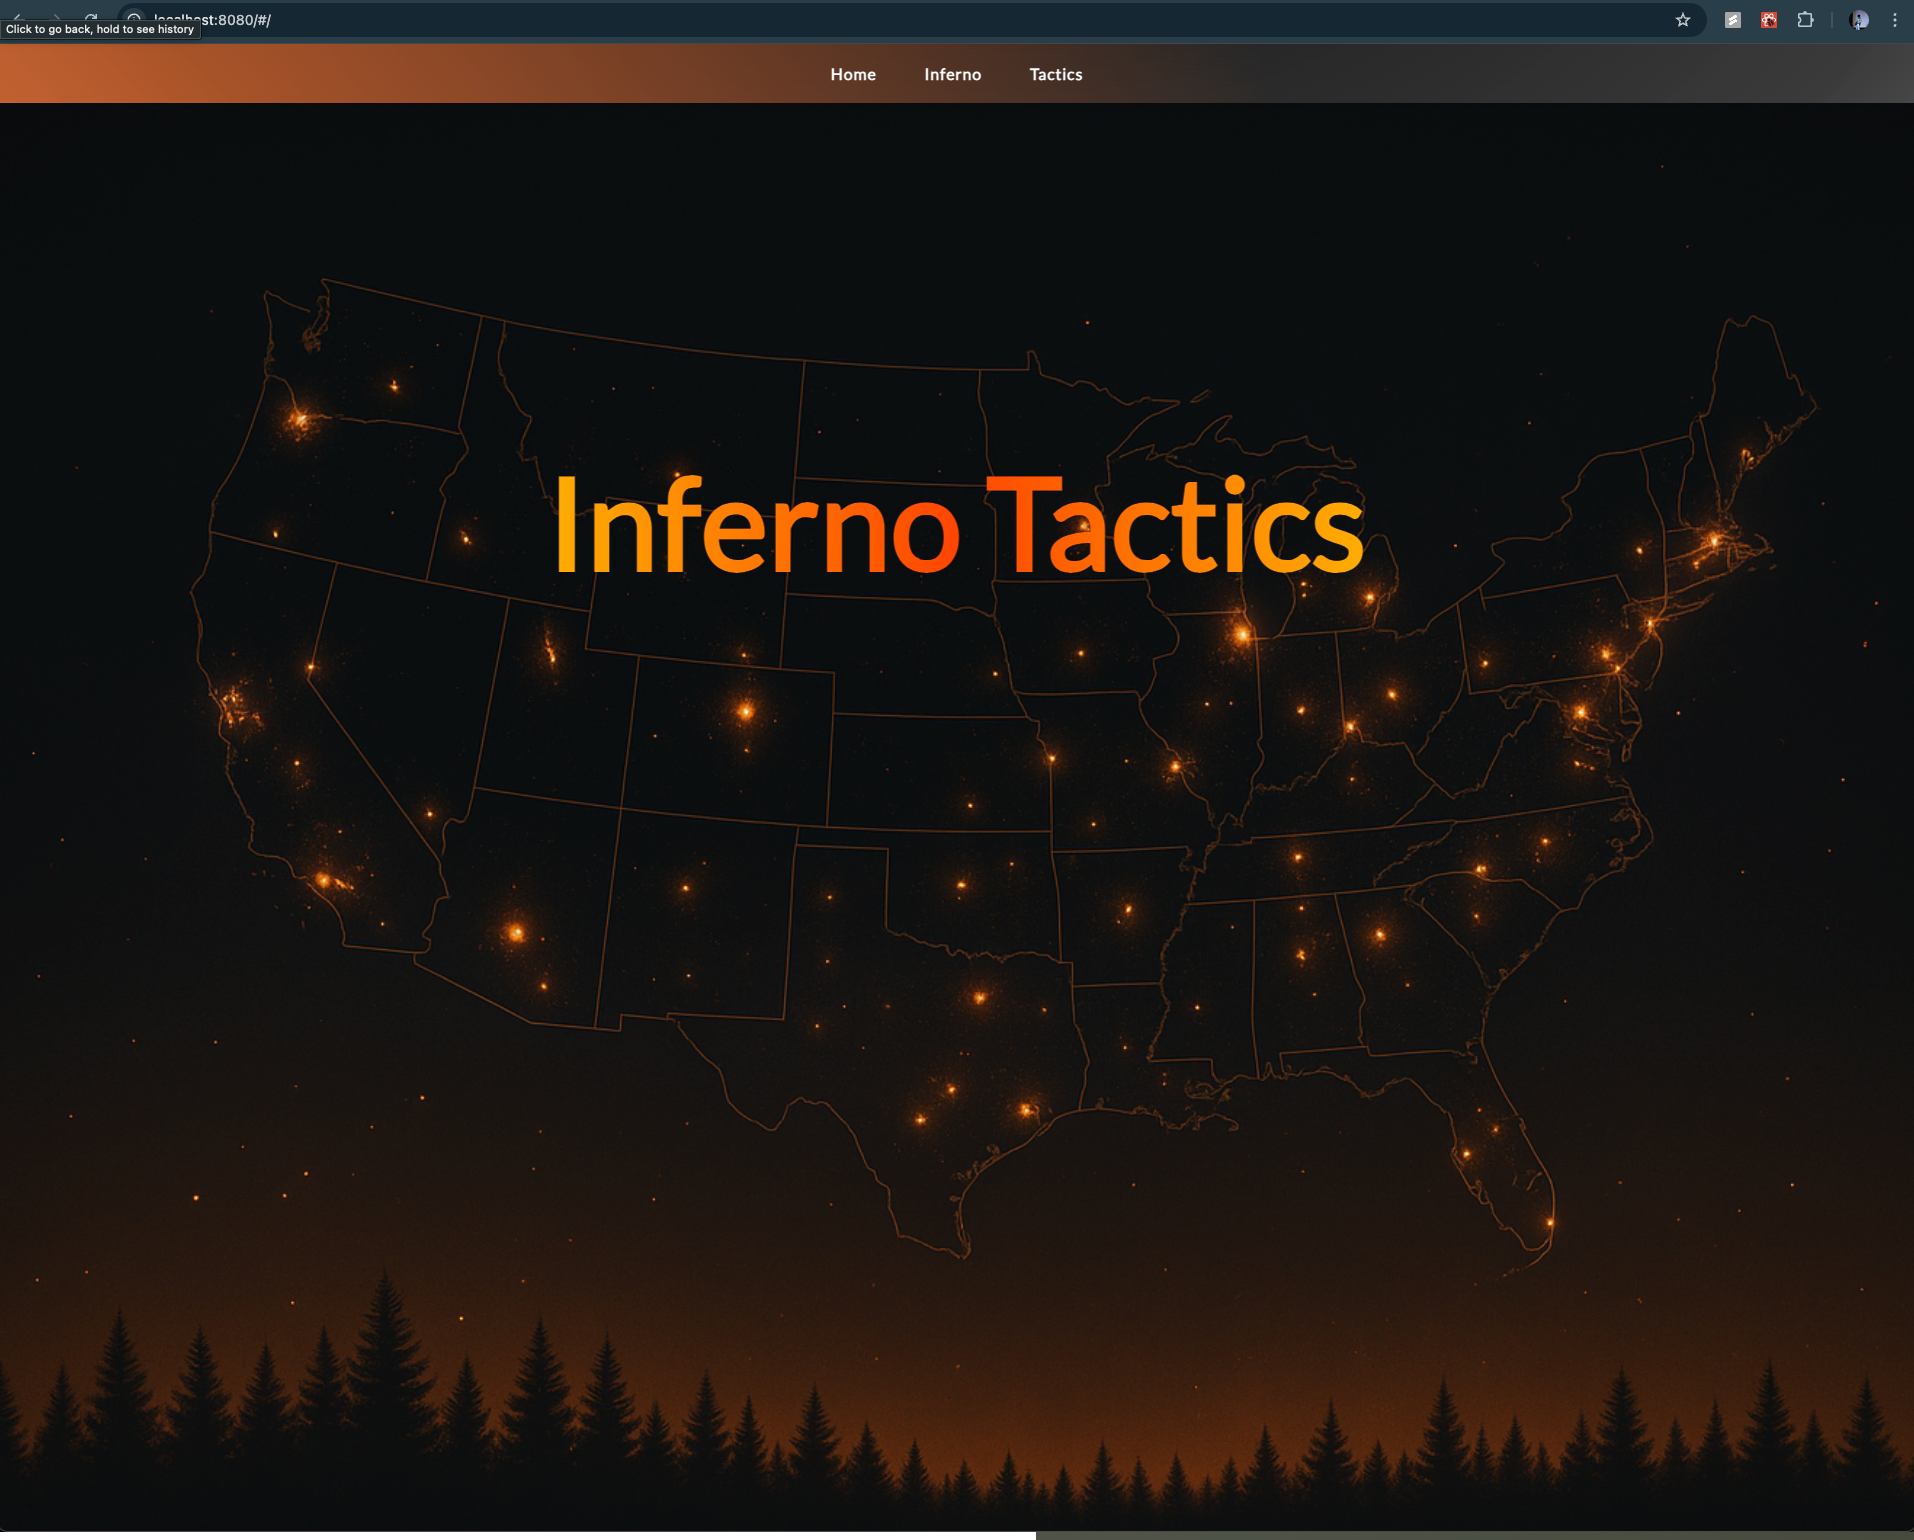
\includegraphics[width=0.5\textwidth]{home.png}
    \caption{Web Application Home Page}
    \end{figure}

    \begin{figure}[H]
        \centering
        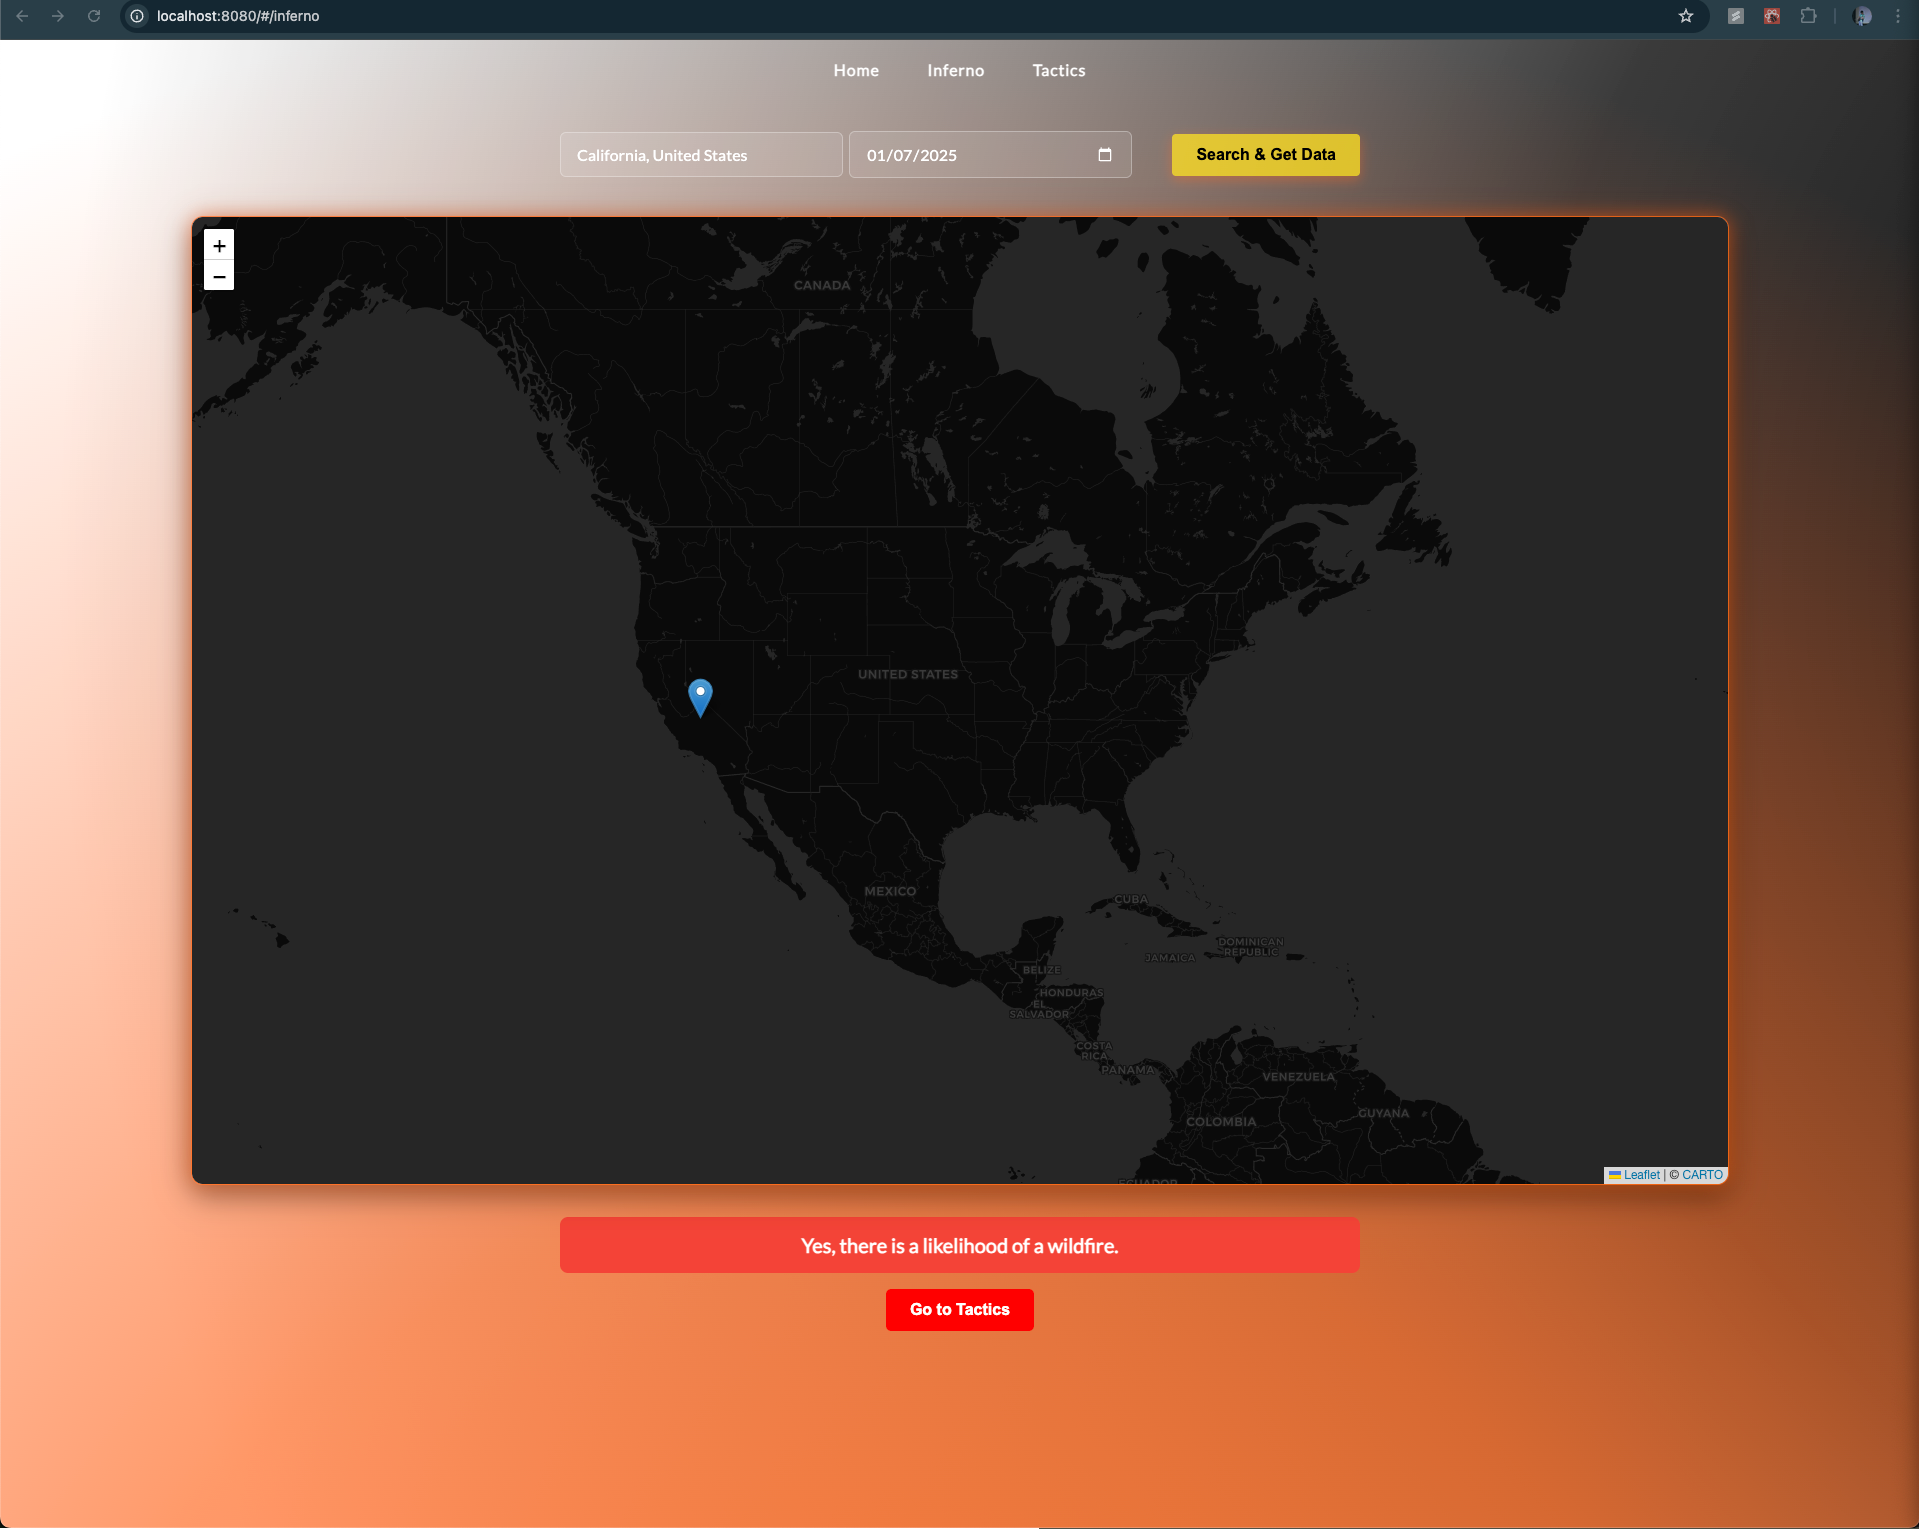
\includegraphics[width=0.5\textwidth]{inferno.png}
        \caption{Inferno Prediction Page}
        \end{figure}

        \begin{figure}[H]
            \centering
            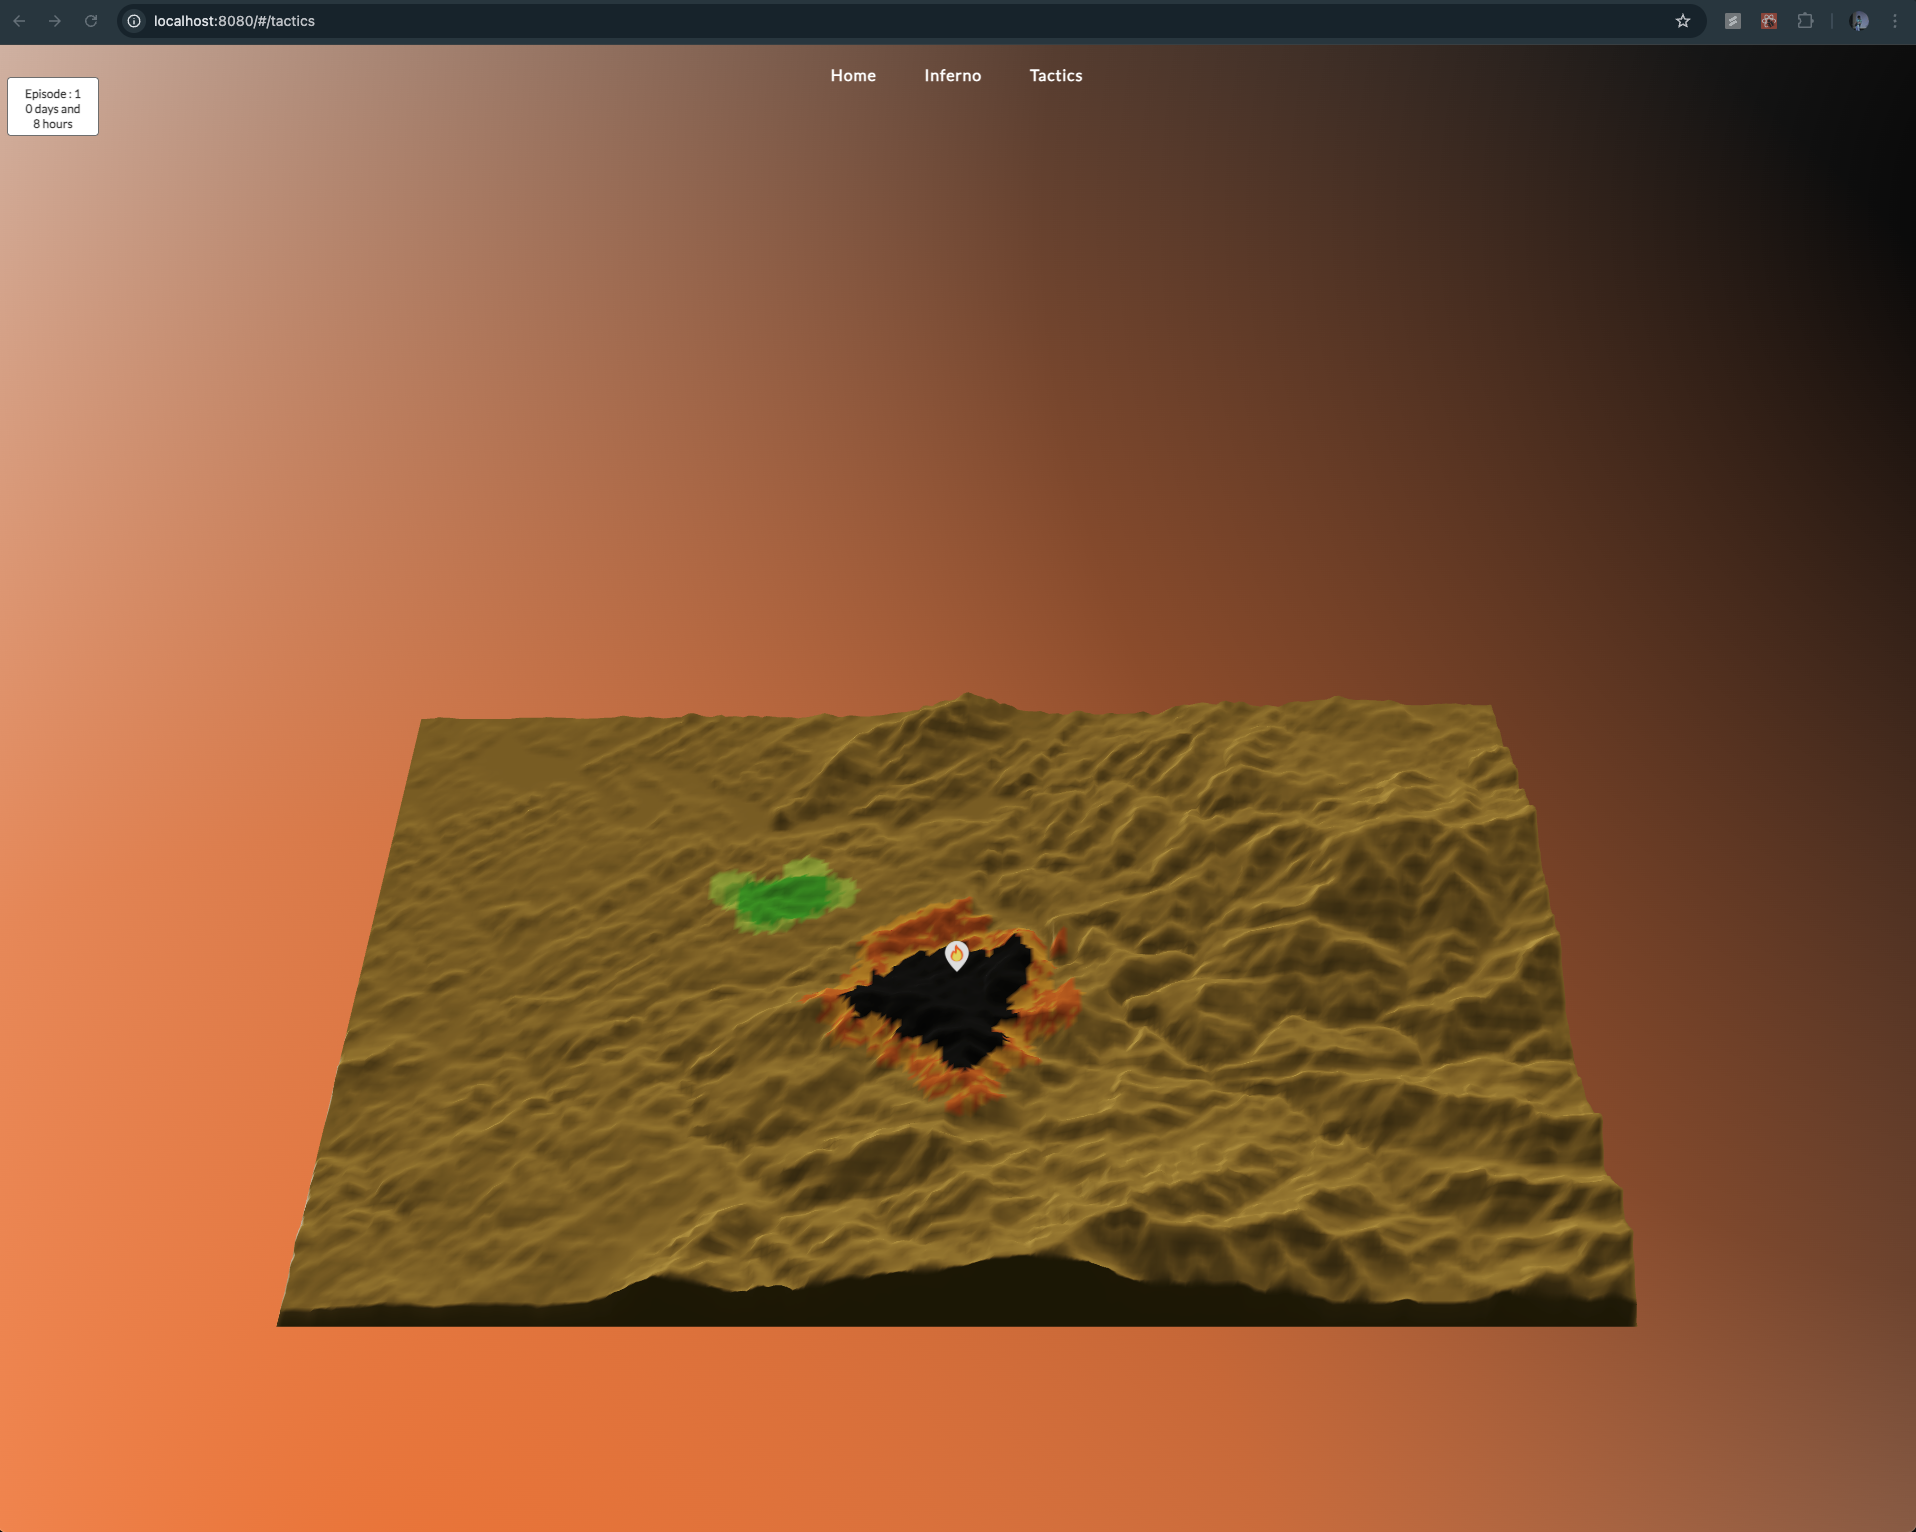
\includegraphics[width=0.5\textwidth]{tactix.png}
            \caption{Tactics Mitigation Page}
            \end{figure}
\begin{itemize}
    \item \textbf{Input Location:} Specify geographic coordinates (latitude and longitude) or use an interactive map to select a region of interest.
    
    \item \textbf{Select Date Range:} Choose a future date or date range for wildfire risk assessment.
    
    \item \textbf{View Prediction Results:} Receive a binary prediction (fire/no fire) along with a confidence score indicating the likelihood of wildfire occurrence.
\end{itemize}

\noindent
If a wildfire is predicted with high confidence, the application automatically triggers the following workflow:

\begin{enumerate}
    \item \textbf{Data Acquisition:} The system fetches elevation data from SRTM and land cover data from MODIS for the specified location.
    
    \item \textbf{Environment Generation:} Using the acquired geodata, the application dynamically creates a simulation environment with dimensions of 1200×800 grid cells (representing a physical area of 120,000×80,000 meters with a heightmap maximum elevation of 10,000 meters).
    
    \item \textbf{Mitigation Simulation:} The pre-trained reinforcement learning agent is deployed in this environment to demonstrate optimal fire suppression strategies.
    
    \item \textbf{Interactive Exploration:} Users can observe the agent's recommended actions, adjust parameters such as wind conditions or resource availability, and explore alternative scenarios.
\end{enumerate}

\subsection{Technical Implementation}
The web application is built using modern web technologies:

\begin{itemize}
    \item \textbf{Frontend:} React.js with Three.js for 3D visualization
    
    \item \textbf{Backend:} Flask server that handles prediction requests and coordinates with the Google Earth Engine for geodata retrieval
    
    \item \textbf{Model Deployment:} TensorFlow Serving for the deep learning prediction model and a custom server for the reinforcement learning policies
    
    \item \textbf{Data Pipeline:} Automated workflow that processes user inputs, generates predictions, and prepares simulation environments
\end{itemize}

\noindent
The integration with our simulation environment allows for seamless transition from prediction to action planning. Once the environment is loaded with the relevant geographic data, users can visualize potential fire spread patterns and explore different mitigation approaches before committing resources in the real world.

\subsection{Practical Applications}
This web application transforms our research into a practical tool for various stakeholders:

\begin{itemize}
    \item \textbf{Emergency Management Teams:} Can use the platform for proactive planning and resource allocation based on predicted fire risks.
    
    \item \textbf{Fire Departments:} May leverage the simulation capabilities to train personnel on optimal response strategies for specific geographic contexts.
    
    \item \textbf{Land Management Agencies:} Can identify high-risk areas and implement preventive measures such as controlled burns or firebreak construction.
    
    \item \textbf{Research Community:} Can utilize the platform to test new wildfire models or adaptation strategies in a realistic virtual environment.
\end{itemize}

\noindent
By providing this accessible interface to our AI-driven wildfire prediction and mitigation system, we aim to bridge the gap between advanced research and practical application in the field of disaster management.

\section{Future Work}

While the current stage of the project has successfully established the foundational architecture and demonstrated promising initial results, several key enhancements are planned to extend the system's capabilities, realism, and impact. These future steps are outlined below.

\subsection{Meta-Reinforcement Learning for Adaptation}
A crucial enhancement to our system will be the integration of \textbf{Meta-Reinforcement Learning (Meta-RL)} capabilities. Wildfire environments are characterized by constant change—variations in weather patterns, fuel conditions, terrain types, and fire behavior make each wildfire event unique. Traditional RL agents often struggle to generalize when faced with environments that differ significantly from their training distribution.

\begin{itemize}
\item \textbf{Rapid Adaptation:} Meta-RL frameworks will enable our agents to quickly adapt to new, previously unseen environmental conditions without extensive retraining. This is particularly valuable for wildfire management, where conditions can change rapidly during a single incident.

\item \textbf{Transfer Learning Across Environments:} By framing wildfire mitigation as a meta-learning problem, we can train agents that learn "how to learn" optimal strategies for different fire scenarios, rather than learning fixed policies for specific conditions.

\item \textbf{Context-Aware Decision Making:} Meta-RL algorithms like Model-Agnostic Meta-Learning (MAML) and Reptile will allow our agents to infer the current environmental dynamics from limited observations and adapt their strategies accordingly.

\item \textbf{Continual Improvement:} As the system encounters more wildfire scenarios, the meta-learning component will progressively improve its adaptation capabilities, making the entire system more robust to environmental variability.
\end{itemize}

\noindent
The implementation of Meta-RL will be particularly beneficial when expanding beyond our current single helitack agent to include multiple agent types. Each agent class can leverage meta-learning to specialize in certain environmental contexts while maintaining adaptability across a range of conditions.

\subsection{Hierarchical Reinforcement Learning}
Our current system models a single firefighting strategy (helitack) through a single-agent RL approach. We aim to expand this to a multi-tiered control system using \textbf{Hierarchical Reinforcement Learning (HRL)}. In this framework:

\begin{itemize}
\item A high-level policy will choose between multiple mitigation strategies, such as deploying fire trucks, helitacks, or constructing firebreaks.
\item Low-level policies (sub-agents) will handle the specific execution of each strategy.
\item This approach will allow the agent to operate at both strategic and tactical levels, improving overall adaptability and efficiency.
\end{itemize}

\subsection{Multi-Agent Coordination}
In real-world wildfire mitigation, coordination between multiple response units is essential. As a next step, we plan to implement a \textbf{multi-agent system} that extends beyond our current single helitack agent:

\begin{itemize}
\item Each agent represents a distinct firefighting unit (e.g., ground crew, fire truck, fixed-wing aircraft, drone reconnaissance).
\item Agents may have overlapping but not identical observation spaces and action sets.
\item Coordination and communication protocols will be explored using frameworks like MADDPG (Multi-Agent Deep Deterministic Policy Gradient).
\end{itemize}

\subsection{Policy Transfer to Real Geographies}
Currently, our training environments are based on simulated data generated from real-world maps. As the models mature, we intend to:

\begin{itemize}
\item Fine-tune trained agents on historical wildfire case studies (e.g., California, Australia).
\item Leverage transfer learning techniques to adapt policies across varying terrain and climate conditions.
\item Validate agent performance using satellite data and fire event records.
\end{itemize}

\subsection{Real-Time Decision Support Tool}
A major goal of this project is to build a decision-support interface that can assist emergency response teams. Future development includes:

\begin{itemize}
\item Deploying the simulation as a cloud-based tool with real-time updates.
\item Allowing human operators to interact with the system and adjust RL agent recommendations.
\item Incorporating user feedback to dynamically re-train or fine-tune models.
\end{itemize}

\subsection{Explainability and Trust in RL Decisions}
As we deploy RL in high-stakes decision-making scenarios, building trust in the agent's choices is critical. Planned work includes:

\begin{itemize}
\item Developing visualization techniques to explain agent decisions.
\item Analyzing action trajectories and counterfactuals to understand failure cases.
\item Using interpretable RL models or post-hoc explainability tools to aid human oversight.
\end{itemize}

\subsection{Integration with Government and NGO Systems}
Long-term, we envision this system being seamlessly integrated with wildfire management platforms used by:

\begin{itemize}
\item Government agencies (e.g., CAL FIRE, NASA FIRMS) for real-time fire spread insights and mitigation planning.
\item NGOs involved in environmental protection and disaster response for prioritizing interventions and resource deployment.
\item Research organizations focused on climate-resilient infrastructure and AI-powered disaster forecasting.
\end{itemize}

\noindent
As a final output, the system generates a concise, human-readable one-page report using a fine-tuned large language model (LLM), summarizing the fire's behavior, estimated spread, and recommended actions. This empowers field officers and policy makers to make fast, informed decisions without needing to interpret complex geospatial data.

\noindent
By continuing to refine and scale this pipeline, we aim to offer a robust, intelligent, and accessible decision-support framework to help tackle one of the world's most urgent environmental threats.

\section{Bonus: Project Management Tool}
For this project, we utilized \textbf{Trello} as our project management tool to ensure structured progress tracking and clear communication. The project was divided into several milestones including data exploration, proposal drafting, basic and advanced model implementations, training, testing, and final presentation preparations.

Since our collaboration spanned both the reinforcement learning (RL) and deep learning (DL) parts of the project, both Trello boards were linked. Weekly tasks were clearly documented, enabling effective contribution tracking and synchronization between team members.

Key milestones included:

\begin{enumerate}
\item[-] Project initialization
\item[-] Data gathering and preprocessing
\item[-] Initial model development
\item[-] Advanced model enhancements
\item[-] Training and validation of models
\item[-] Evaluation and final adjustments
\end{enumerate}

\subsection{Project Management Screenshots}
Below are screenshots showcasing our Trello-based project management efforts:

\begin{figure}[H]
\centering
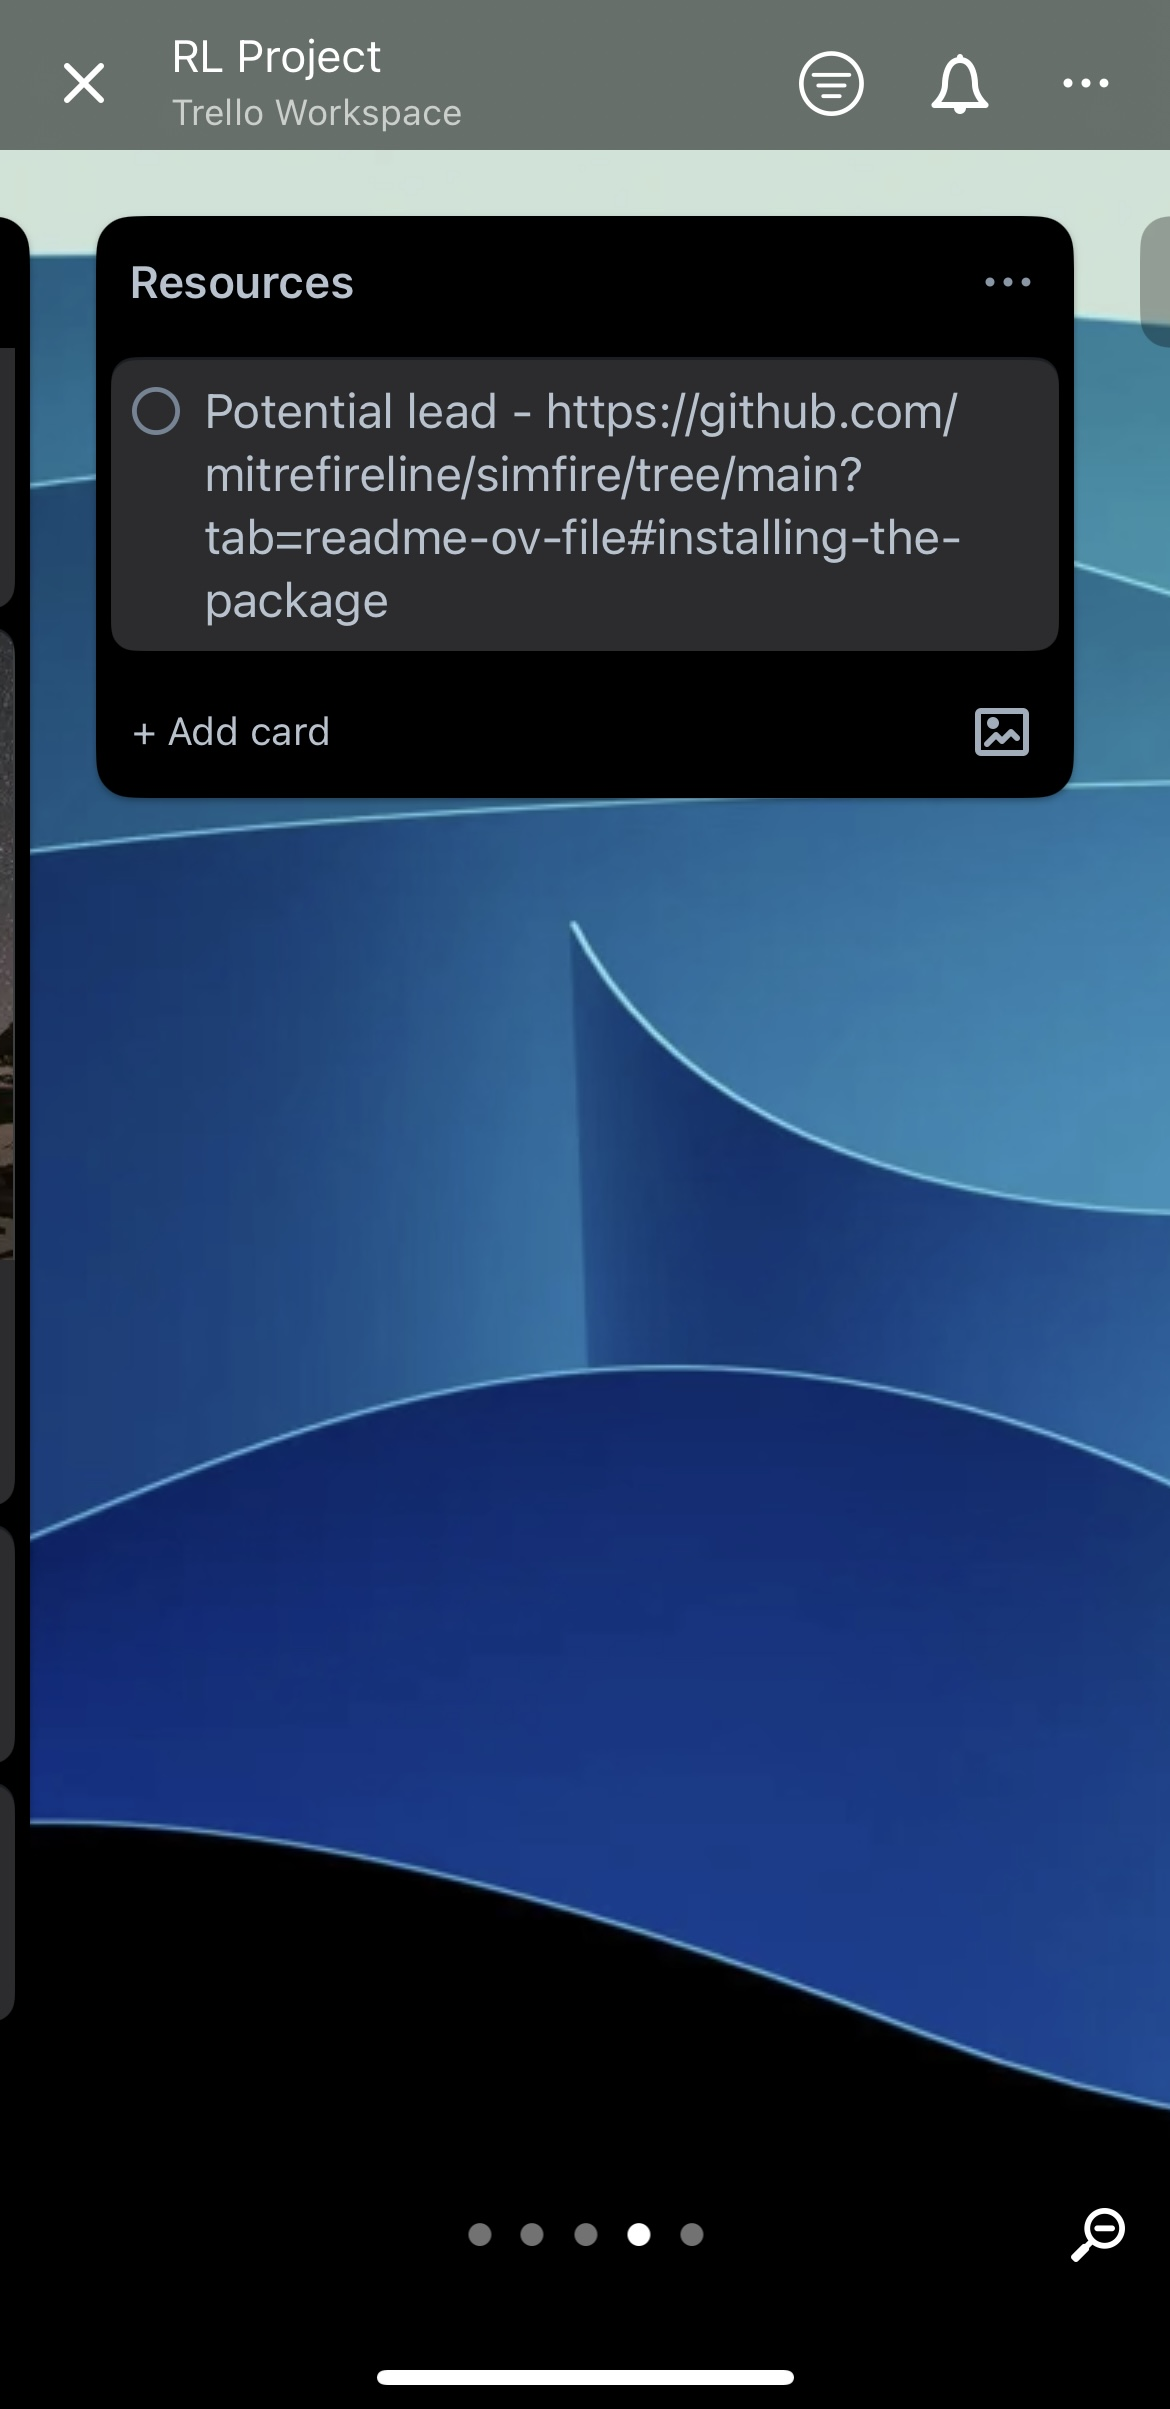
\includegraphics[width=0.2\textwidth]{1.jpg}
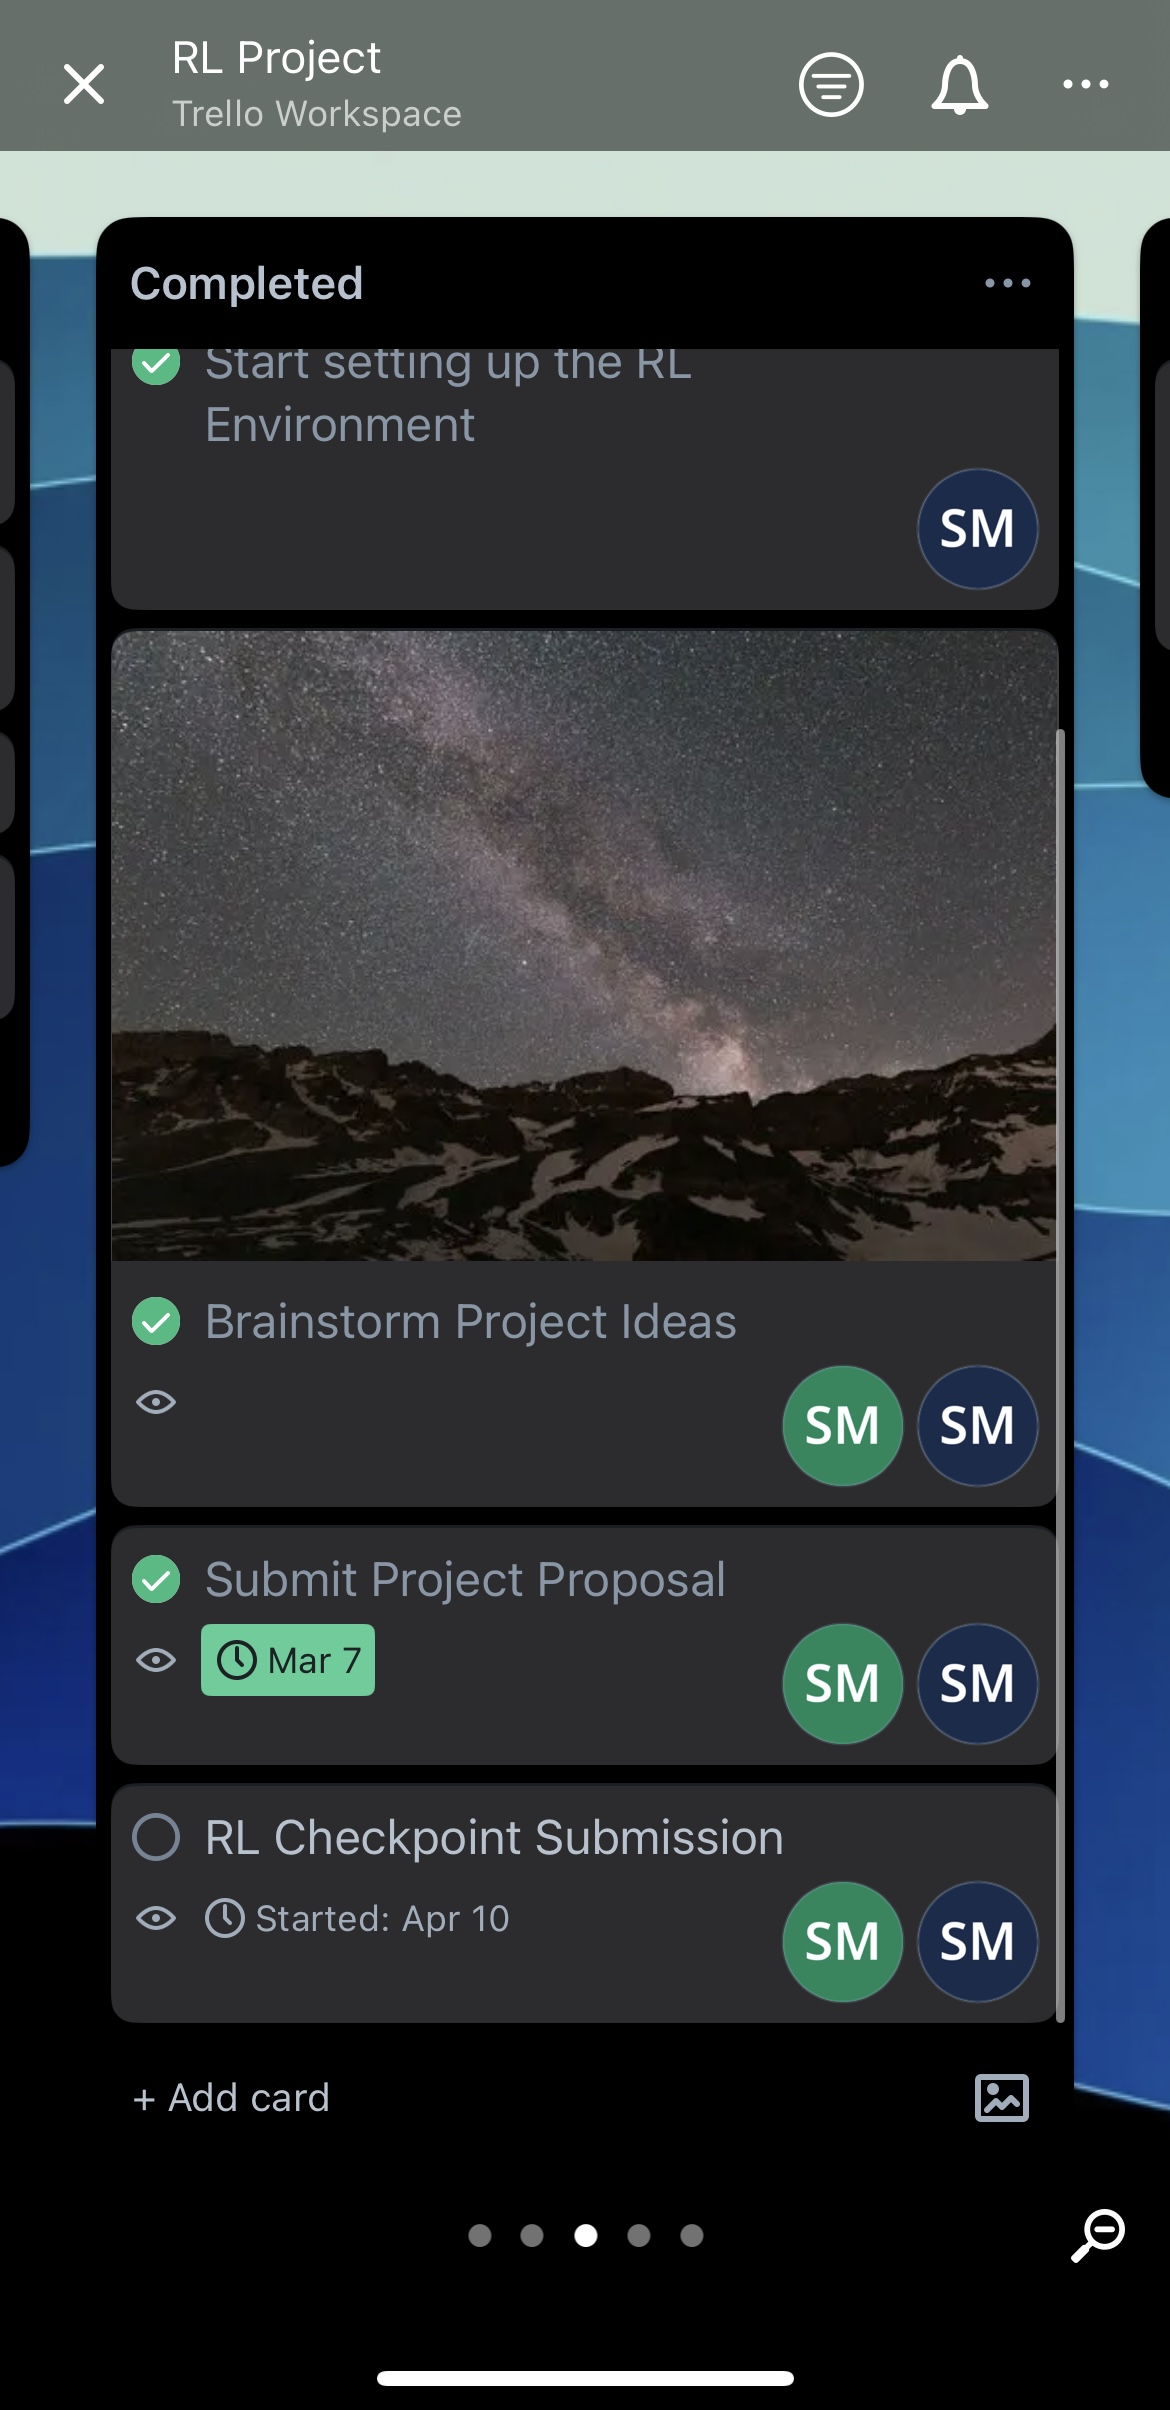
\includegraphics[width=0.2\textwidth]{2.jpg}
\end{figure}
\vspace{-0.7cm}
\begin{figure}[H]
\centering
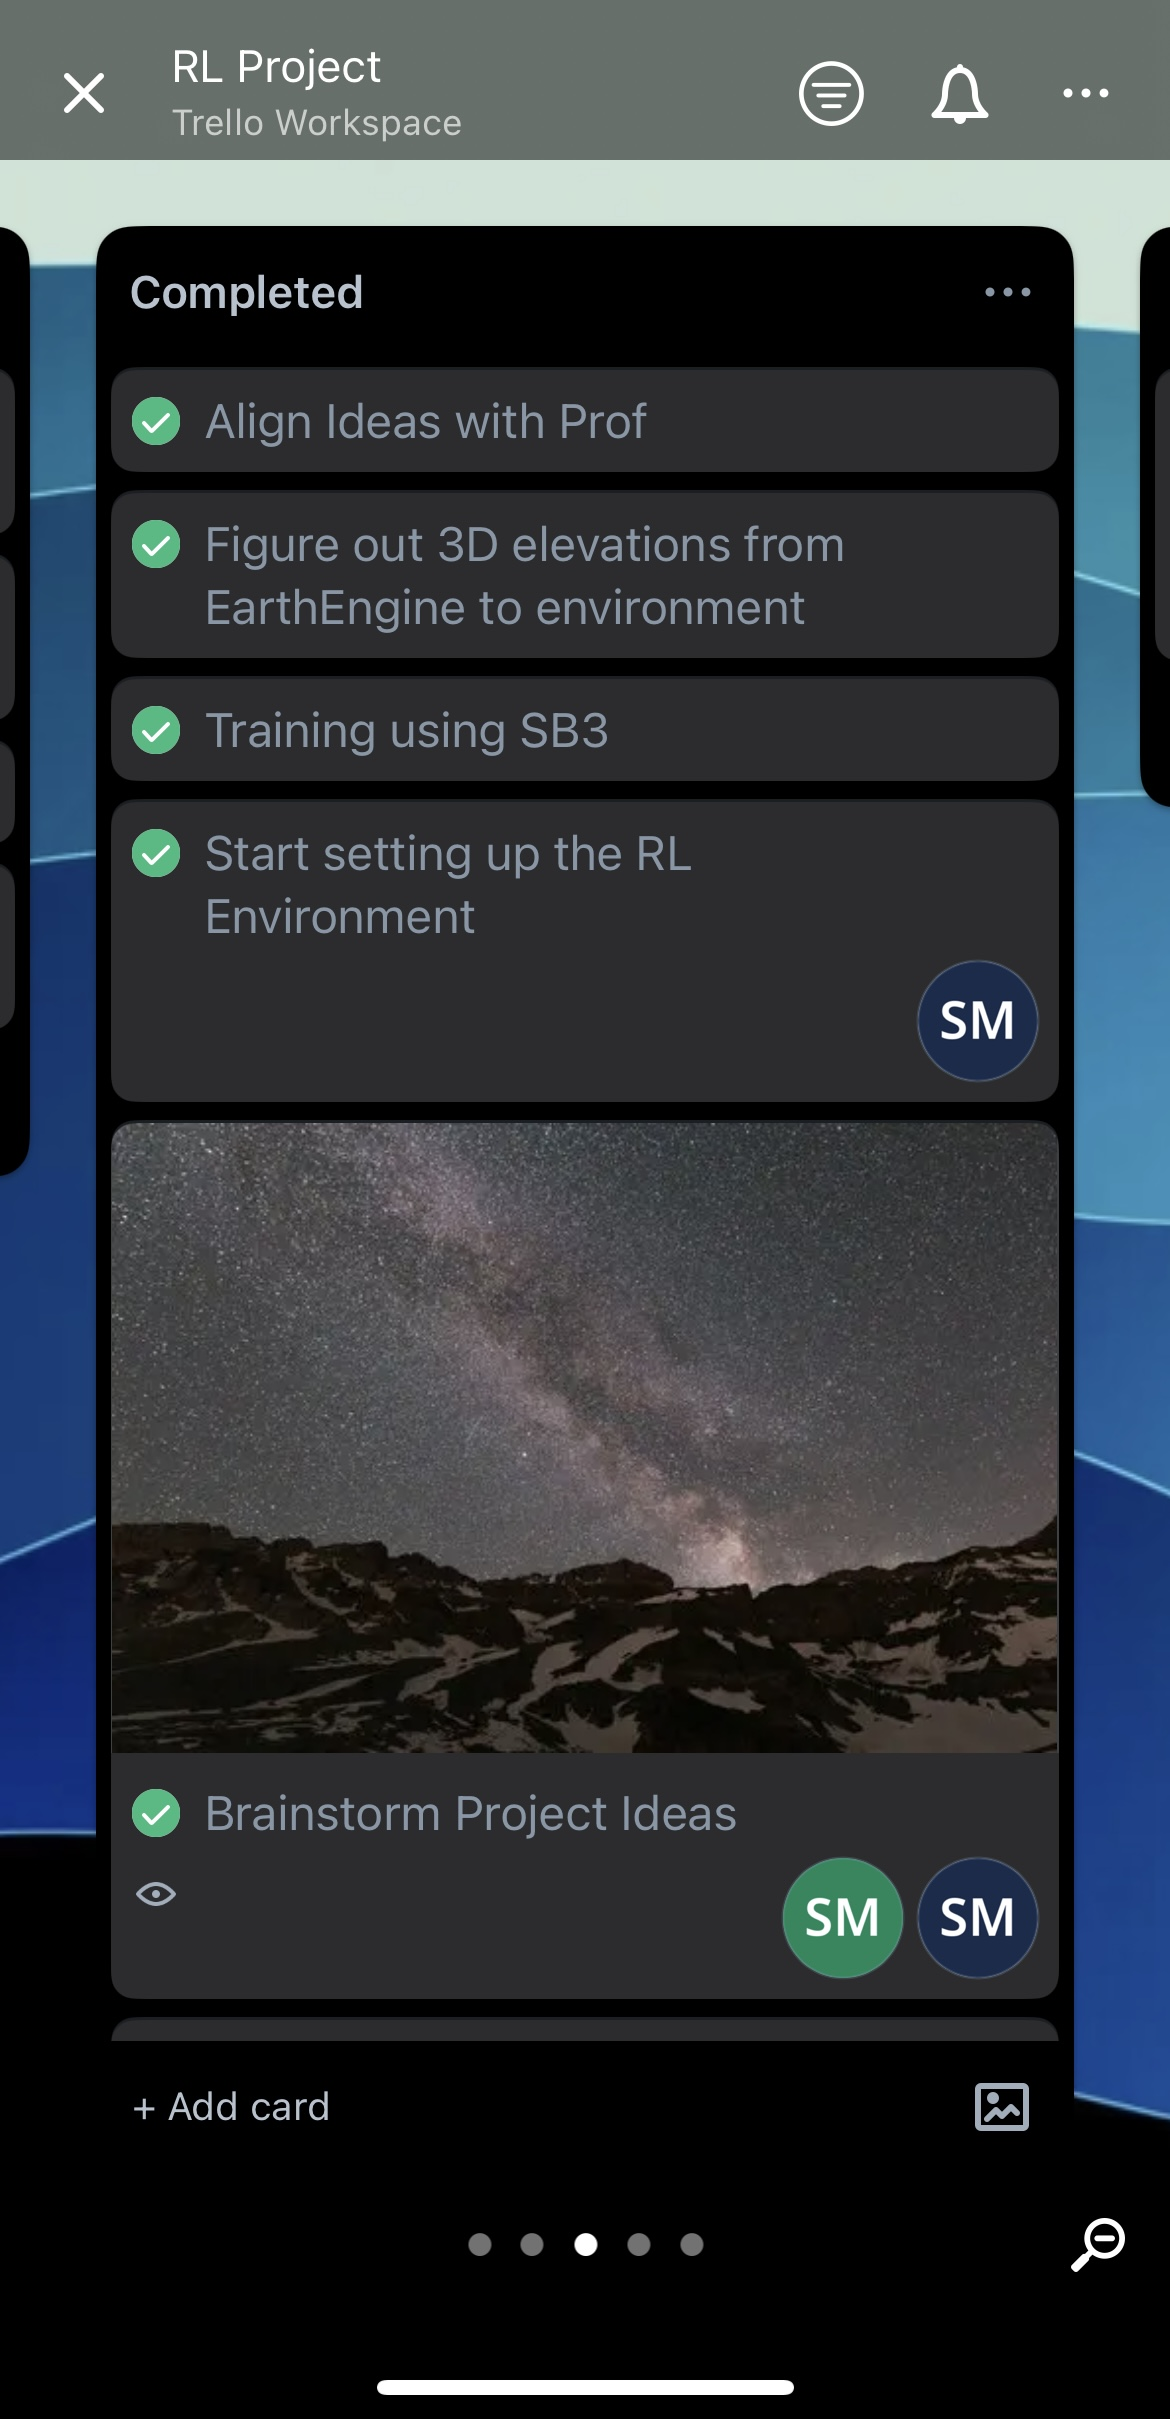
\includegraphics[width=0.2\textwidth]{3.jpg}
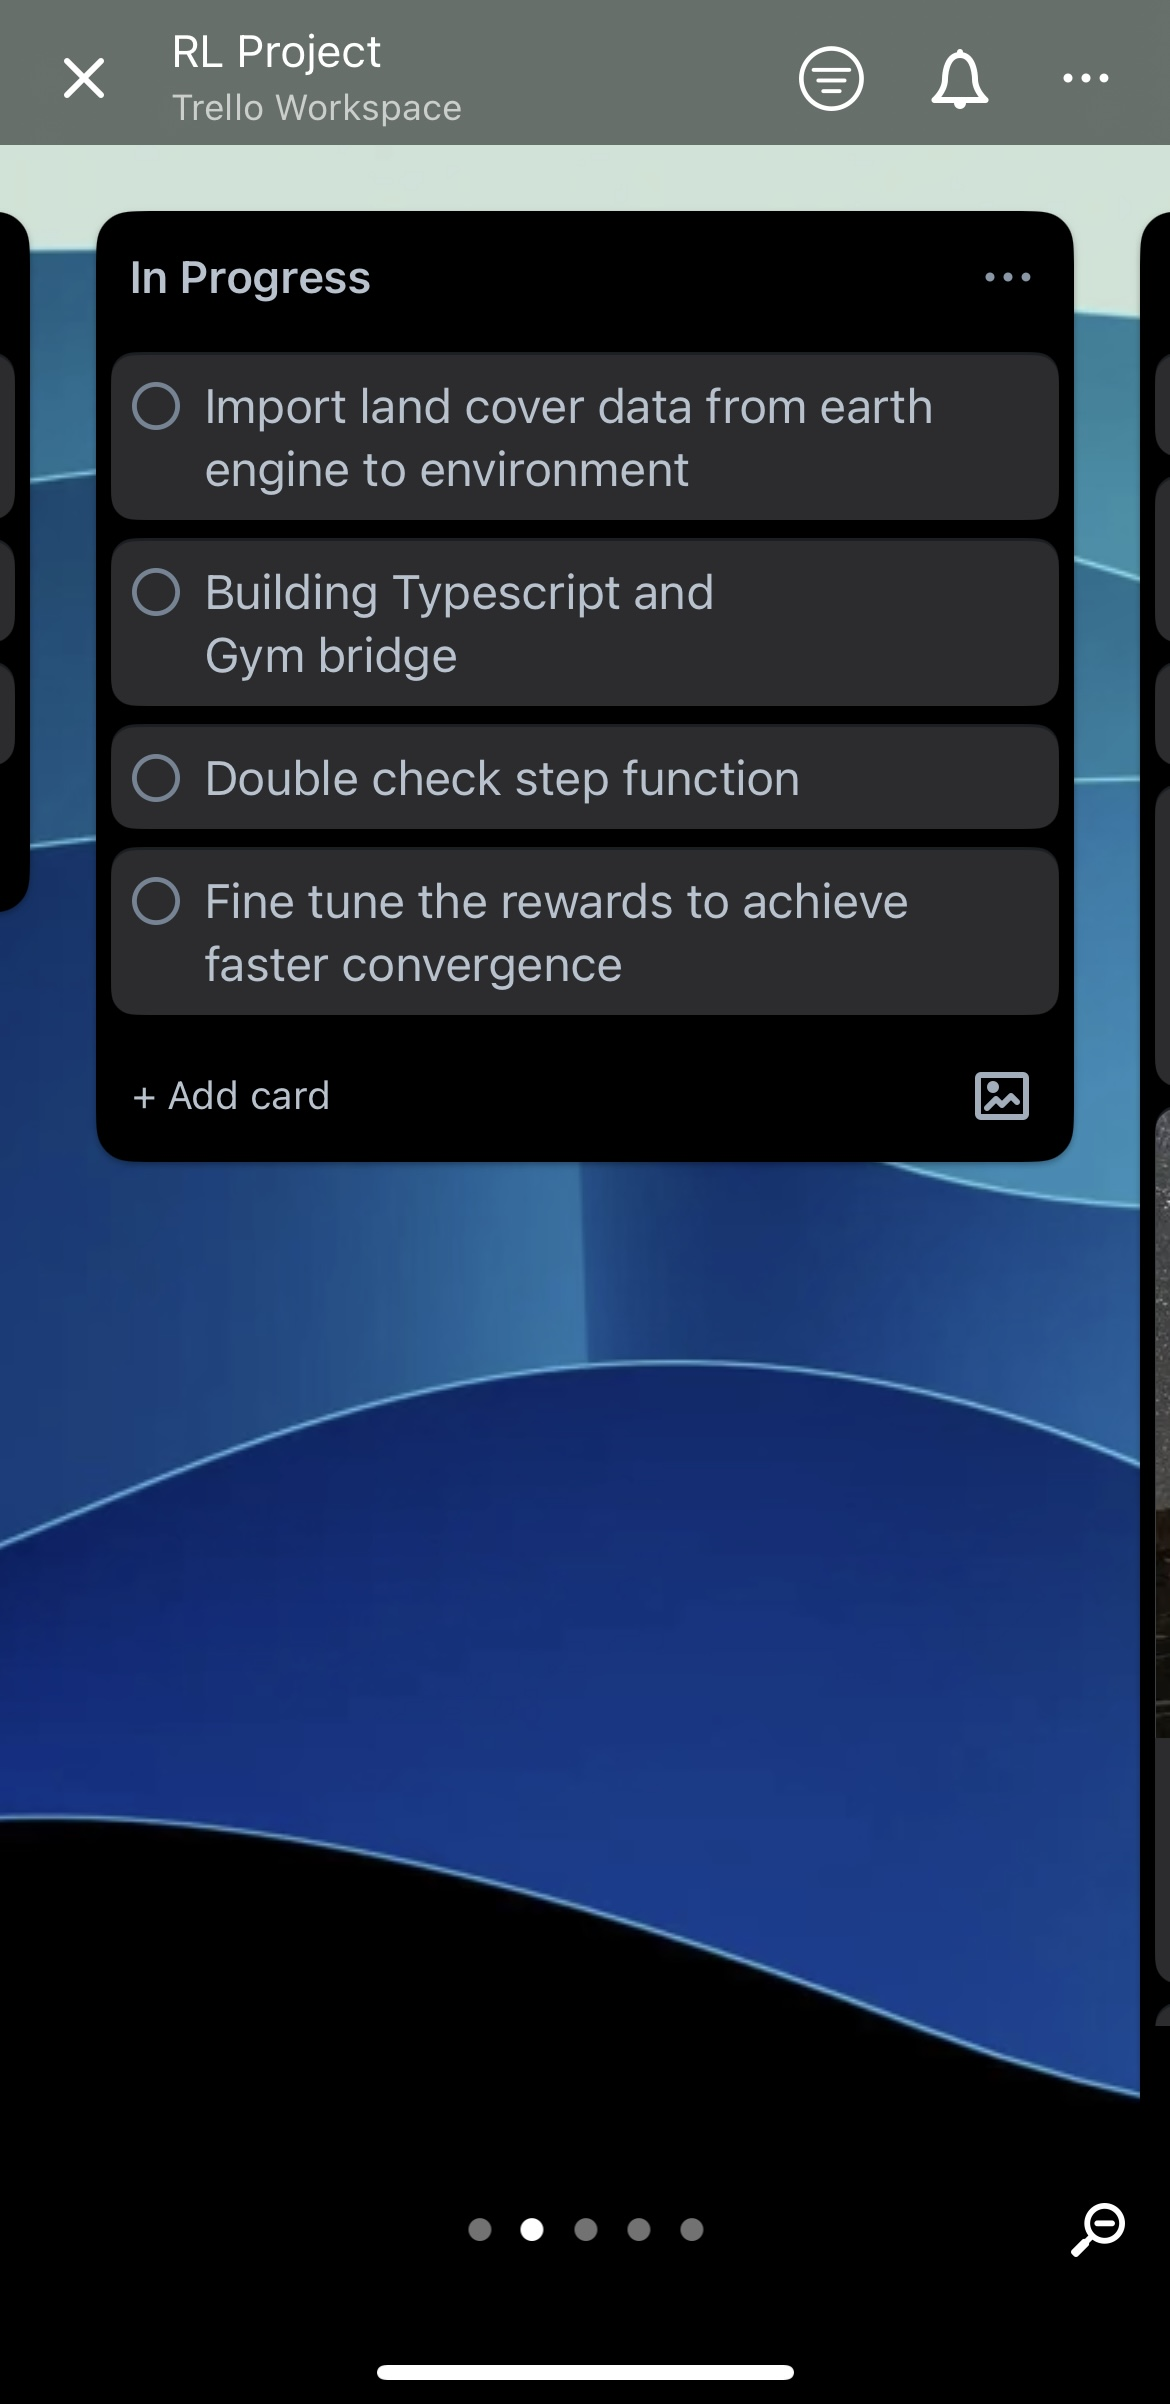
\includegraphics[width=0.2\textwidth]{4.jpg}
\end{figure}
\vspace{-0.7cm}

\begin{figure}[H]
    \centering
    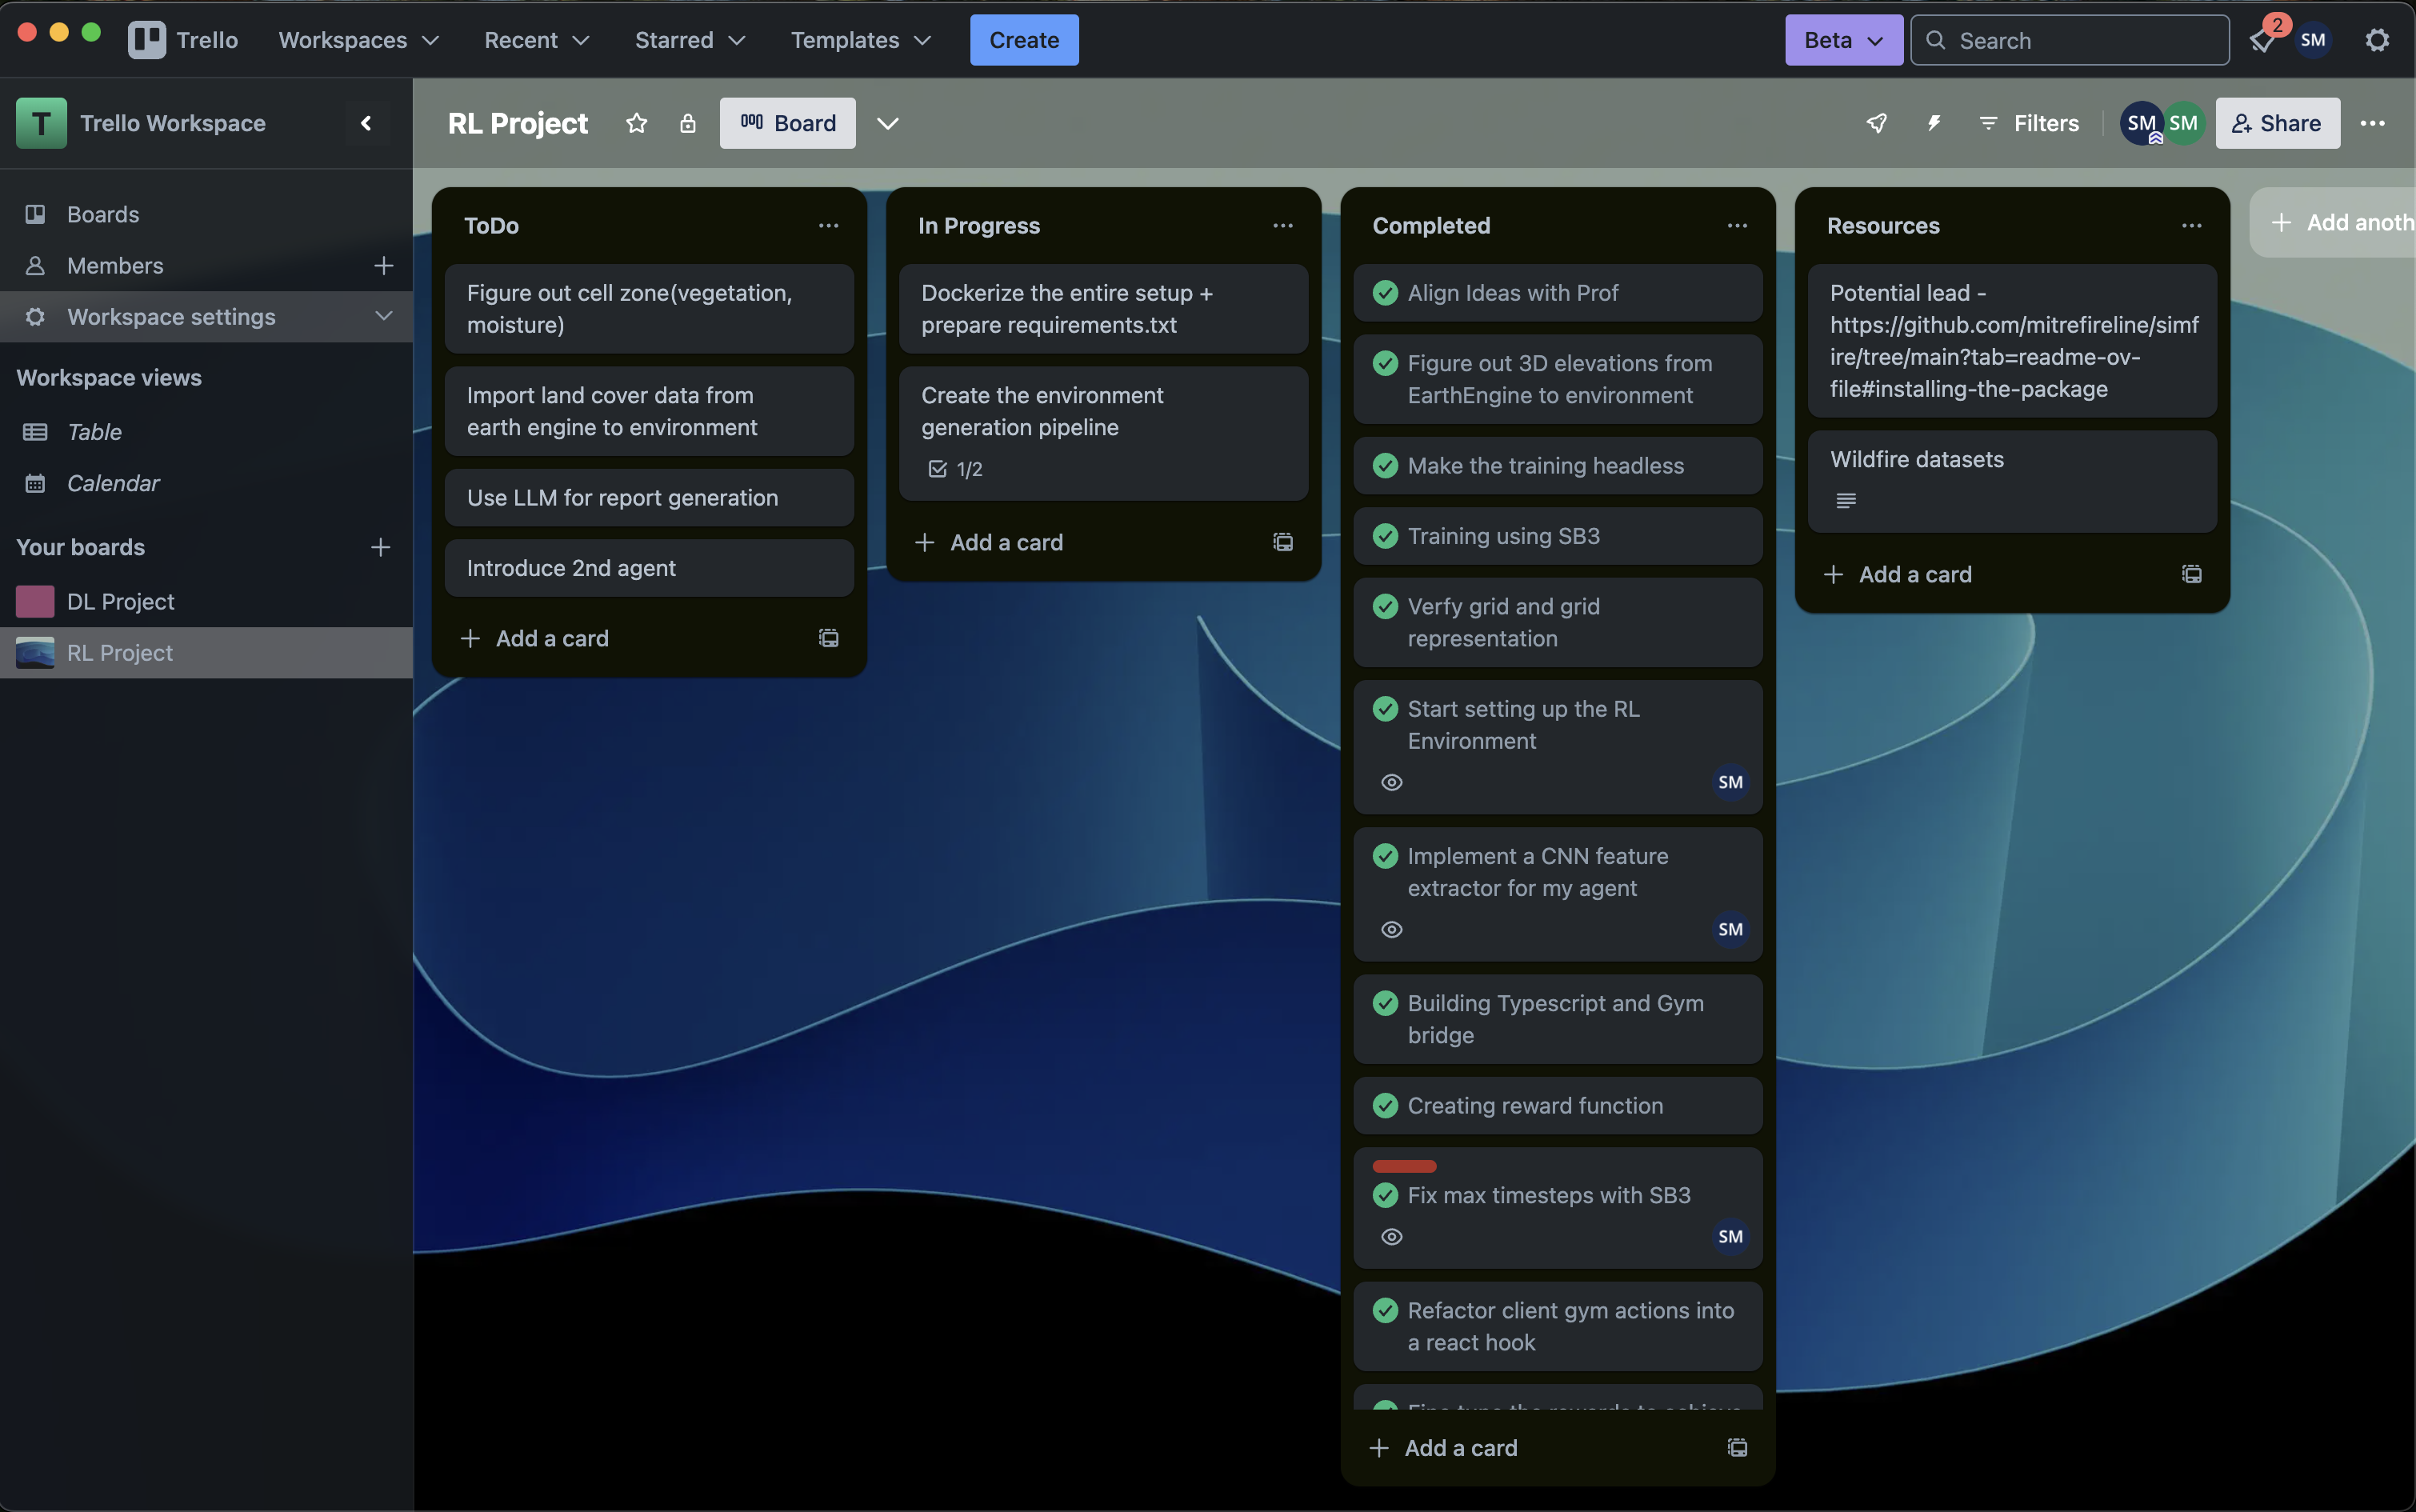
\includegraphics[width=0.5\textwidth]{trello_rl.png}
    \caption{Trello Dashboard}
    \end{figure}

\vspace{-0.3cm}
\noindent\textbf{Trello Board URL:} \\
\texttt{https://trello.com/b/pBNt9VwL/rl-project}

\vspace{0.3cm}
\noindent\textbf{GitHub Repository:} \\
\texttt{https://github.com/ShauryaMathur/inferno-tactix/tree/wildfire-env}

\subsection{GitHub Commit History}
\hspace{-0.4cm}Below is a snapshot of our git commit history demonstrating ongoing collaboration and iterative development:

\begin{figure}[H]
\centering
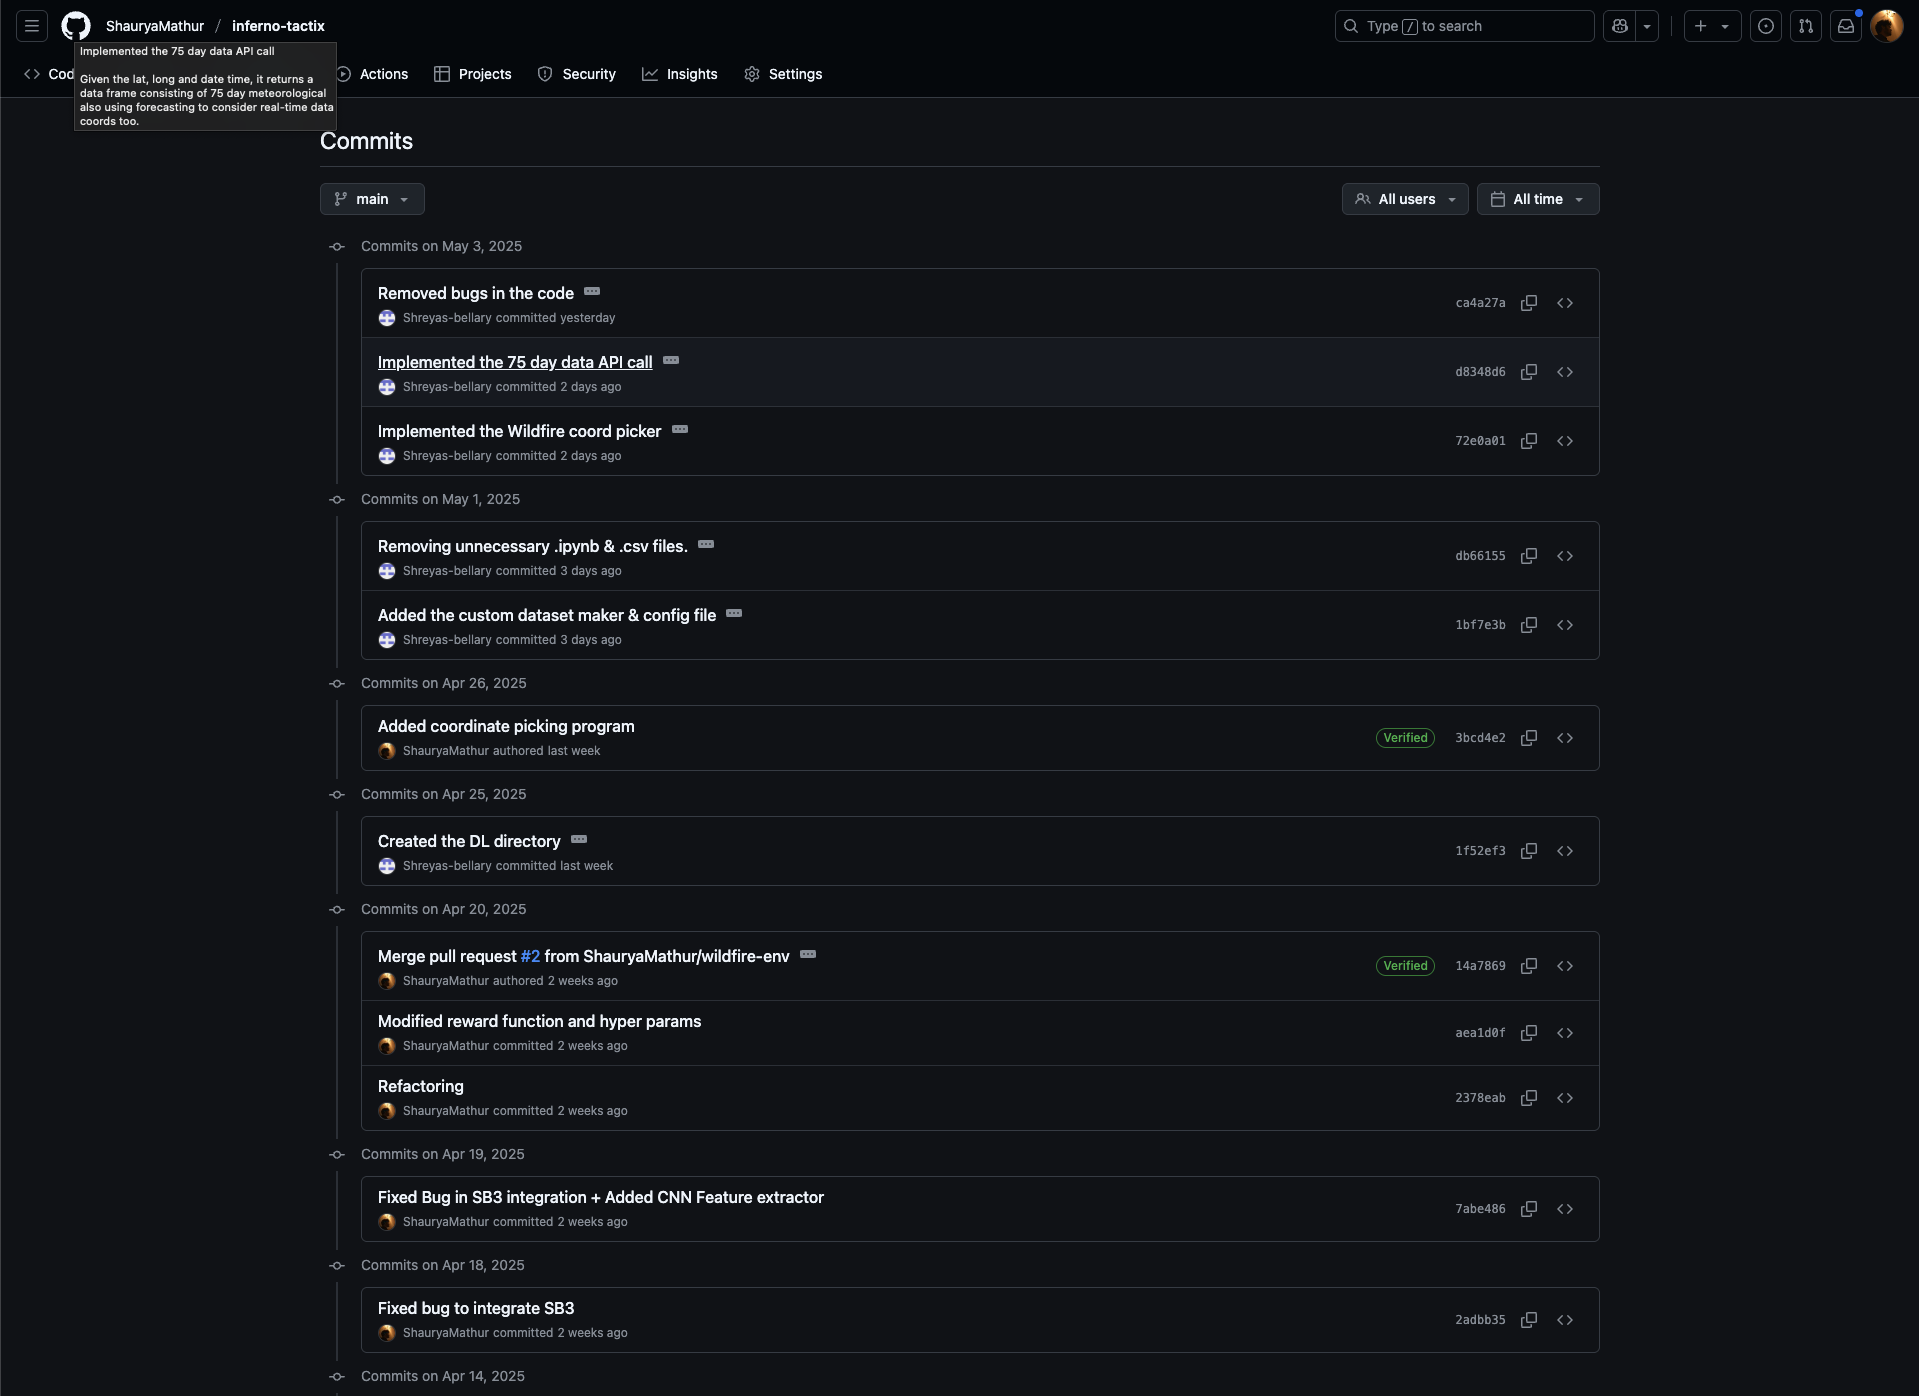
\includegraphics[width=0.5\textwidth]{git1.png}
\caption{Git commit history (part 1)}
\end{figure}

\begin{figure}[H]
    \centering
    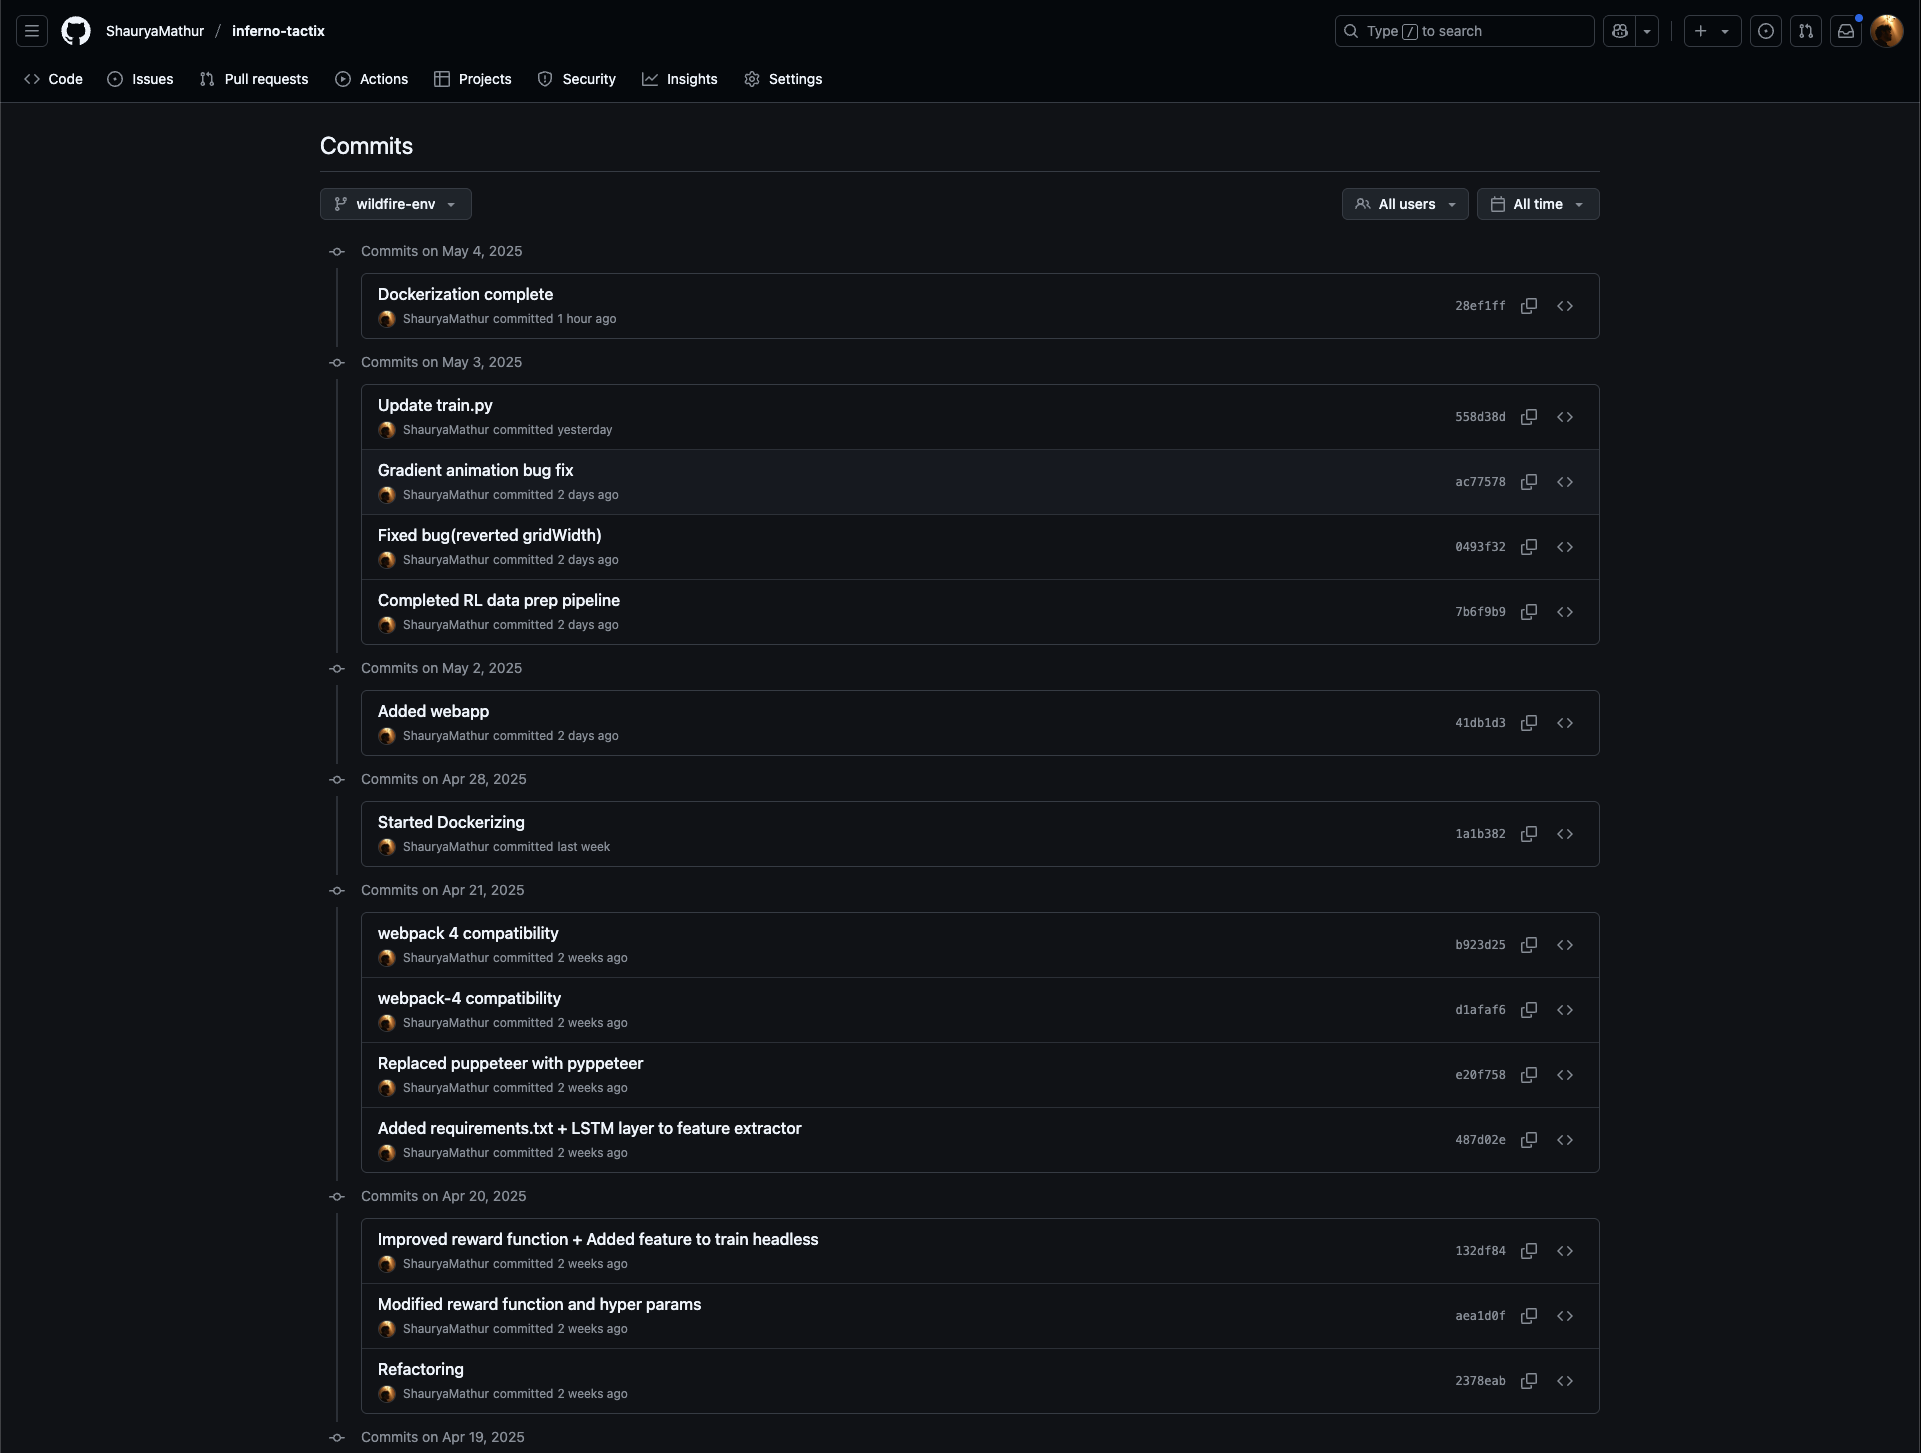
\includegraphics[width=0.5\textwidth]{git2.png}
    \caption{Git commit history (part 2)}
    \end{figure}

\vspace{0.4cm}
\begin{thebibliography}{00}
\bibitem{b1} https://github.com/amanbasu/wildfire-detection
\bibitem{b2} https://code.earthengine.google.com/
\bibitem{b3} https://wildfire.concord.org/
\bibitem{b4} https://github.com/concord-consortium/wildfire-model/tree/master
\bibitem{b5} U.S. Geological Survey, \emph{Landsat 8 (L8) Data Users Handbook}, U.S. Geological Survey, 2019. [Online]. Available: \url{https://landsat.usgs.gov/landsat-8}
\bibitem{b6} Y. Zhao, M. Chen, and S. Kumar, ``A Comprehensive Review of Deep Learning Techniques for Wildfire Detection in Satellite Images,'' \emph{IEEE Access}, vol. 9, pp. 10523--10539, 2021.
\bibitem{b7} M. Pereira and G. H. A., ``Active Fire Detection in Landsat-8 Imagery: A Large-Scale Dataset,'' GitHub, 2023. [Online]. Available: \url{https://github.com/pereira-gha/activefire}
\bibitem{b8} https://earthengine.google.com/
\bibitem{b9} https://medium.com/@AlexanderObregon/building-real-time-applications-with-python-and-websockets-eb33a4098e02
\bibitem{b10} https://stable-baselines3.readthedocs.io/en/master/modules/ppo.html
\end{thebibliography}

\end{document}